\documentclass[a4paper,DIV=10]{scrartcl}


\usepackage{graphicx}
\usepackage{hyperref}
\usepackage{float}


\newcommand{\op}[6]{
  \subsection{#1}
  #2
  
  \subsubsection*{Signature:}
  \ \ #3
  
  \subsubsection*{Context element (selectedEObject):}     
  \ \ #4
  
  \subsubsection*{Additional parameters:} 
  #5
  
  \subsubsection*{Precondition:}    
  \ \ #6
  
  \subsubsection*{Implementation in EMF Henshin:}
}

\newcommand{\cond}[3]{
	\subsection{#1}
	\label{subsec:#2}
	#3
}


\author{\textbf{Technical Report}\\
\hfill\\
Michaela Rindt, Timo Kehrer, Udo Kelter, Pit Pietsch\\
Software Engineering Group\\
University of Siegen}

\title{Rules for Edit Operations in Class Diagrams}

\date{rev. 2012-01-06}

% \title{
% A Catalog of Basic Edit Operations\\ for UML Class Models\\ \hfill \\
% \LARGE{Informal Specifications and Rule-based Implementations with EMF Henshin \hfill \\ \hfill \\}
% }

\begin{document}
\maketitle

\newpage
\tableofcontents

\newpage
\section{Introduction}

This technical report specifies edit operations for UML
class diagrams.
 We assume that the class diagrams are represented as
Ecore objects using the EMF technology.
 Each operation is specified as follows:

\begin{enumerate}
\item by a short informal description from a users' point
   of view

\item by a suggested signature of a method which
   implements this edit operation, and an informal
   description of the parameters in this signature

\item by the preconditions (informally specified) which must
   hold to successfully perform the edit operation

\item by an implementation of this edit operation as a
   Henshin transformation rule, which acts as a formal,
   precise specification.

\end{enumerate}

The main emphasis is on the formal specifications using
Henshin. These edit rules can be translated into software
which detects applications of these edit operations in 
a difference between two models, s. \cite{KeKT2011ASE}
for details.


\paragraph{Coverage of the UML Metamodel.} This catalog of
edit rules covers only the more important concepts of UML
class diagrams. For example, details such as
ValueSpecifications in multiplicities are not covered.
Future versions of this document will extend the set of
covered modelling concepts.

\paragraph{Used UML Metamodel.}
The creation of edit rules for class diagrams is based
on an internally developed UML Metamodel which is highly
truncated in comparison to the UML2.0 standard of the OMG \cite{OMG}.
This internal UML Metamodel is restricted to class diagrams only.
A concrete design difference lies e.g. in the construction of associations:
UML2.0 associations contain property elements which refer to the
target and source of the association. In the SiDiff UML Metamodel
an UMLAssociation contains so called UMLAssociationEnds wich refer
to the source and target of an association.
This is just one example of how these meta models differ.
If you are interested in how the SiDiff UML Metamodel is built,
please take a look at the according link under the references \cite{SiDiff-UML}.

\paragraph{Tooling.}
The edit operations were designed
with EMF-Henshin and EMF-Refactor.

EMF-Henshin provides a graphical user interface for
defining such edit operation, whereas EMF-Refactor is an
extension with which one can define preconditions to the
actual transformation process.

More Information about EMF-Henshin can be found under
their project page
\cite{Henshin}. To find more information about
EMF-Refactor visit the EMF-Refactor project page
\cite{Refactor}.



\subsection{Design Rules for Edit Operations} 

Some edit operations are obviously needed, e.g. operations
for creating and deleting model elements. This catalog
contains many additional operations, mostly ``move
operations'', which are not strictly necessary, but
convenient. An example of this is the operation which
moves a class into another package; instead of moving the
class, it could be deleted and reconstructed from scratch
in the other package.

Whenever possible, we have avoided to use undefined or default values. For
example, when creating a class, its name must be specified immediately in a parameter.

Another design decision was that each edit operation should be
implementable by one Henshin transformation.
 There are some model modifications which could be
implemented in different ways.

 Since the creation of Henshin transformations for UML is
still work in progress, this catalog of edit operations is
not yet complete and sometimes discretionary.




\subsection{Notations}

In general, every transformation consists of two files:
the (graphical) diagram file and the (more technical)
Henshin-graph file. In the latter, one can create
TransformationUnits which will define the execution
sequence of rules in different ways. In some cases of the
following transformations you will find excerpts of such
unit graphs for a better understanding.

Notations like 'nameValue/newName' show first the
parameter name used in the mainUnit of the graph-file and
secondly the placeholder name of the element in the
diagram-file.

Most conditions are very similar and are therefore just
listed once under the section 'Conditions'. You will find
a reference to these under relevant sections. 

Please note that the conditions are not yet complete.





\section{Conditions}
With EMF Refactor and Henshin conditions can be designed either as
'initialCheck', 'finalcheck' or as 'execute'.
\\\\
Where initial- and finalcheck serve as preconditional check, the 'execute'-type
is the actual transformation which does the modification.

Note, with finalchecks one designes the 'negative' case which is not wanted for
the execution to be run - or in other words: the finalcheck must NOT match for
the 'execute' to be run.

%----------Pre:checkOtherNames----------------------------------------
\cond
{Precondition: checkOtherNames}
{checkOtherNames}
{This precondition is a 'finalcheck'. checkOtherNames
will match if an element (here: UMLClass) with the same name like
in the propagated value of 'newName' exists under the selected context (here:
UMLPackage) and therefore prevent the actual transformation process.
\\\\
In other words: the finalcheck mustn't match if one wants the corresponding
'execute' (here e.g. createClass or editClassName) to be run.}

\begin{figure}[H]
  \centering
  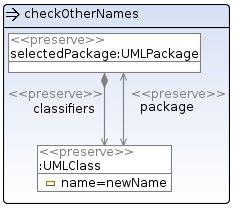
\includegraphics[width=0.4\textwidth]{pics/cond_checkOtherNames.png}
  \caption{checkOtherNames}
  \label{checkOtherNames}
\end{figure}
%----------Pre:checkOppositeAggregationKind---------------------------
\cond
{Precondition: checkOppositeAggregationKind}
{checkOppositeAggregationKind}
{still to be implemented}
%----------Pre:checkInheritanceCycle----------------------------------
\cond
{Precondition: checkInheritanceCycle}
{checkInheritanceCycle}
{still to be implemented}


\newpage
\section{Packages}
%----------createPackageInModel----------------------------------------
\op
{createPackageInModel}
{Adds a package in a model / under the root element}
{createPackageInModel(Model selectedEObject, String idValue, String nameValue)}
{The model providing the container for the newly created package.}
{
\begin{itemize}
 \item idValue/newID: The identifier of the newly created package 
 \item nameValue/newName: The name of the newly created package
\end{itemize}
}
{There is no package whose name equals the parameter-value of 'newName' (see
\ref{subsec:checkOtherNames})}
{A new package and references to and from
the model will be created. 'selectedModel', as it is shown in the picture,
is a placeholder for the concrete Model which will be delivered via mappings
of the selectedEObject. Also a default value 'public' for the visibility feature
will be set.} \begin{figure}[H]
  \centering
  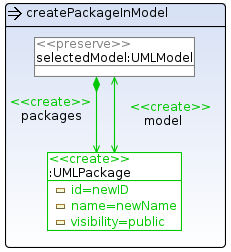
\includegraphics[width=0.4\textwidth]{pics/createPackageInModel.png}    
  \caption{createPackageInModel}
  \label{createPackageInModel}  
\end{figure}

%----------createPackageInPackage----------------------------------------
\op
{createPackageInPackage}
{Adds a package in a package}
{createPackageInPackage(Package selectedEObject, String idValue, String nameValue)}
{The package providing the container for the newly created package.}
{
\begin{itemize}
 \item idValue/newID: The identifier of the newly created package 
 \item nameValue/newName: The name of the newly created package
\end{itemize}
}
{There is no package whose name equals the parameter-value of 'newName' (see
\ref{subsec:checkOtherNames})}
{A new package and references to and from
the super package will be created. 'selectedPackage', as it is shown in the
picture, is a placeholder for the concrete super package which will be delivered
via mappings of the selectedEObject. Also a default value 'public' for the visibility feature
will be set.}
\begin{figure}[H]
  \centering
  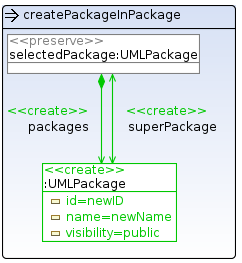
\includegraphics[width=0.4\textwidth]{pics/createPackageInPackage.png}
  \caption{createPackageInPackage}
  \label{createPackageInPackage}
\end{figure}

%----------deletePackage----------------------------------------
\op
{deletePackage}
{Deletes a package}
{deletePackage(Package selectedEObject)}
{The package which should be deleted }
{-}
{-}
{For a better readability this is a simplified version of the
'deletePackage'-transformation and will only cover cases where the
package has no containments and no references to other elements. Such a
complex transformation rule exits but won't be listed here.
\\\\
In this simple version we first of all have to find out from which context type
the selected package should be deleted. For this we have the rule 'containerIsModel', which matches if the
container is a model. If not we can assume that the context is a package since
no other model element can contain a package according to the meta model specification.\\
After we know the context type one of the two variants of the delete-rule
(deletePackageFromModel and deletePackageFromPackage) can be applied.\\\\
Below you can also see the graph of units which explains this process with
an if-then-else structure called 'Conditional Unit'. The selectedEObject is the
placeholder for the context and it will be propagated to the according
parameters in the three rules via the so called 'Parameter Mappings'.

}
\begin{figure}[H]
  \advance\leftskip-1.5cm
  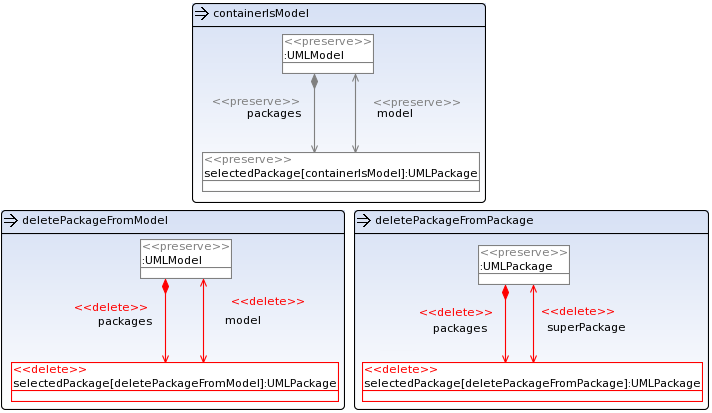
\includegraphics[width=1.2\textwidth]{pics/deletePackage_emptyAndUnreferenced.png}
  \caption{deletePackage}
  \label{deletePackage}
\end{figure}
\begin{figure}[H]
  \centering
  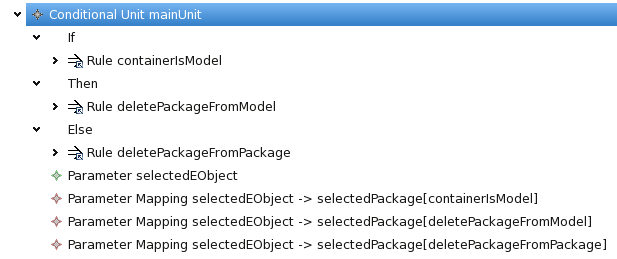
\includegraphics[width=1.0\textwidth]{pics/deletePackage_emptyAndUnreferenced_TreeView.png}
  \caption{deletePackage(UnitView)}
  \label{deletePackage}
\end{figure}
%----------editPackageName----------------------------------------
\op
{editPackageName}
{edits the name of a package}
{editPackageName(Package selectedEObject, String nameValue)}
{The package whose name should be renamed.}
{
\begin{itemize}
 \item nameValue/newName: The new name
\end{itemize}
}
{There is no package whose name equals the parameter-value of 'newName' (see
\ref{subsec:checkOtherNames})}
{The 	\textless\textless create\textgreater\textgreater  -symbol in the image
means that even if the attribute exists its value will be overwritten. 'newName'
is the placeholder for the input name.}
\begin{figure}[H]
  \centering
  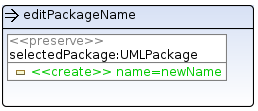
\includegraphics[width=0.4\textwidth]{pics/editPackageName.png}
  \caption{editPackageName}
  \label{editPackageName}
\end{figure}

%----------editPackageVisibility----------------------------------------
\op
{editPackageVisibility}
{edits the visibility of a package}
{editPackageVisibility(Package selectedEObject, Visibility visibilityValue)}
{The package whose visibility should be edited.}
{
\begin{itemize}
 \item visibilityValue/visibility: The new visiblility
\end{itemize}
}
{-}
{The 	\textless\textless create\textgreater\textgreater  -symbol in the image
means that even if the attribute exists its value will be overwritten.
'visibility' is the placeholder for the input visibility.}
\begin{figure}[H]
  \centering
  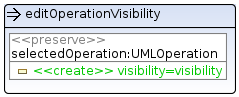
\includegraphics[width=0.4\textwidth]{pics/editPackageVisibility.png}
  \caption{editPackageVisibility}
  \label{addPackage-execute}
\end{figure}

%----------movePackageFromModelToPackage----------------------------------------
\op
{movePackageFromModelToPackage}
{moves a package from a model into package}
{movePackageFromModelToPackage(Package selectedEObject, Package tgt)}
{The package which should be moved.}
{
\begin{itemize}
 \item tgt/targetPackage: the target package
\end{itemize}
}
{There is no package with the same name in the target context (see
\ref{subsec:checkOtherNames})}
{Only the references change}
\begin{figure}[H]
  \centering
  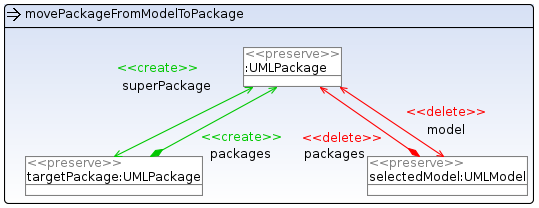
\includegraphics[width=0.8\textwidth]{pics/movePackageFromModelToPackage.png}.
  \caption{movePackageFromModelToPackage}
  \label{movePackageFromModelToPackage}
\end{figure}
%----------movePackageFromModelToPackage----------------------------------------
\op
{movePackageFromPackageToModel}
{moves a package from a package directly under the model}
{movePackageFromPackageToModel(Package selectedEObject, Model tgt)}
{The package which should be moved.}
{
\begin{itemize}
 \item tgt/targetModel: the target model
\end{itemize}
}
{There is no package with the same name in the target context (see
\ref{subsec:checkOtherNames})}
{Only the references change}
\begin{figure}[H]
  \centering
  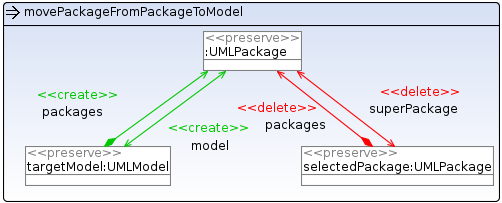
\includegraphics[width=0.7\textwidth]{pics/movePackageFromPackageToModel.png}.
  \caption{movePackageFromPackageToModel}
  \label{movePackageFromPackageToModel}
\end{figure}
%----------movePackageFromModelToPackage----------------------------------------
\op
{movePackageFromPackageToPackage}
{moves a package from a package into another package}
{movePackageFromPackageToPackage(Package selectedEObject, Package tgt)}
{The package which should be moved.}
{
\begin{itemize}
 \item tgt/targetPackage: the target package
\end{itemize}
}
{There is no package with the same name in the target context (see
\ref{subsec:checkOtherNames})}
{Only the references change}
\begin{figure}[H]
  \centering
  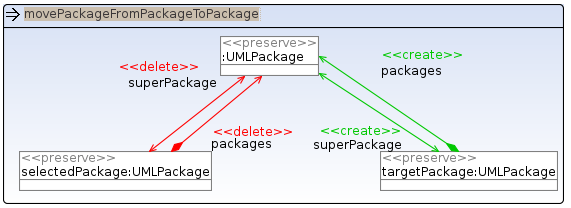
\includegraphics[width=0.9\textwidth]{pics/movePackageFromPackageToPackage.png}.
  \caption{movePackageFromPackageToPackage}
  \label{movePackageFromPackageToPackage}
\end{figure}

\newpage
\section{Classes}
%----------createClass----------------------------------------
\op
{createClass}
{creates a new class}
{createClass(Package selectedEObject, String nameValue)}
{The package providing the container for the newly created class.}
{
\begin{itemize}
 \item nameValue/newName: The name of the newly created class
 \item idValue/newID: The id of the newly created class
\end{itemize}
}
{There is no class whose name equals the parameter-value of 'newName' (see
\ref{subsec:checkOtherNames})}
{Only the name and the id will be set via input data. Visibility, isAbstract and
isFinal will be set with default values as defined with the diagram editor in
the image below.} \begin{figure}[H]
  \centering
  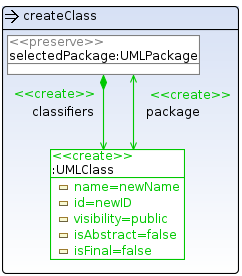
\includegraphics[width=0.4\textwidth]{pics/createClass.png}
  \caption{createClass}
  \label{createClass}
\end{figure}
%----------deleteClass----------------------------------------
\op
{deleteClass}
{Deletes a class}
{deleteClass(Class selectedEObject)}
{The class which should be deleted}
{-}
{-}
{For a better readability this is a simplified version of the
'deleteClass'-transformation and will only cover cases where the class
has no containments and no references to other elements. Such a complex
transformation rule exits but won't be listed here.}
\begin{figure}[H]
  \centering
  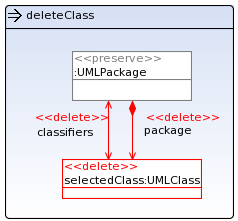
\includegraphics[width=0.4\textwidth]{pics/deleteClass_emptyAndUnreferenced.png}
  \caption{deleteClass}
  \label{deleteClass}
\end{figure}

%----------editClassName----------------------------------------
\op
{editClassName}
{edits the name of a class}
{editClassName(Class selectedEObject, String nameValue)}
{The class whose name should be renamed.}
{
\begin{itemize}
 \item nameValue/someName: The new name
\end{itemize}
}
{There is no class in the same package whose name equals the parameter-value of
'newName' (see
\ref{subsec:checkOtherNames})}
{The \textless\textless create\textgreater\textgreater  -symbol in the image
means that even if the attribute exists its value will be overwritten.
'someName' is the placeholder for the input name.}
\begin{figure}[H]
  \centering
  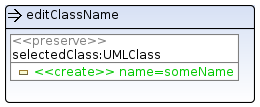
\includegraphics[width=0.45\textwidth]{pics/editClassName.png}
  \caption{editClassName}
  \label{editClassName}
\end{figure}
%----------editClassIsAbstract----------------------------------------
\op
{editClassIsAbstract}
{edits the isAbstract-value of a class}
{editClassIsAbstract(Class selectedEObject, boolean booleanValue)}
{The class whose isAbstract-value should be edited.}
{
\begin{itemize}
 \item booleanValue/bool: The new isAbstract-value
\end{itemize}
}
{-}
{The \textless\textless create\textgreater\textgreater  -symbol in the image
means that even if the attribute exists its value will be overwritten. 'bool'
is the placeholder for the input boolean value.}
\begin{figure}[H]
  \centering
  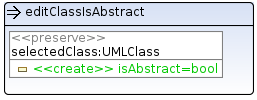
\includegraphics[width=0.45\textwidth]{pics/editClassIsAbstract.png}
  \caption{editClassIsAbstract}
  \label{editClassIsAbstract}
\end{figure}
%----------editClassIsFinal----------------------------------------
\op
{editClassIsFinal}
{edits the isFinal-value of a class}
{editClassIsFinal(Class selectedEObject, boolean booleanValue)}
{The class whose isFinal-value should be edited.}
{
\begin{itemize}
 \item booleanValue/bool: The new isFinal-value
\end{itemize}
}
{-}
{The \textless\textless create\textgreater\textgreater  -symbol in the image
means that even if the attribute exists its value will be overwritten. 'bool'
is the placeholder for the input boolean value.}
\begin{figure}[H]
  \centering
  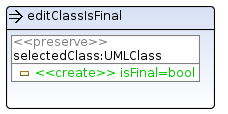
\includegraphics[width=0.40\textwidth]{pics/editClassIsFinal.png}
  \caption{editClassIsFinal}
  \label{editClassIsFinal}
\end{figure}
%----------editClassVisibility----------------------------------------
\op
{editClassVisibility}
{edits the visibility of a class}
{editClassVisibility(Class selectedEObject, Visibility visibilityValue)}
{The class whose visibility should be edited.}
{
\begin{itemize}
 \item visibilityValue/visibility: The new visiblility
\end{itemize}
}
{-}
{The \textless\textless create\textgreater\textgreater  -symbol in the image
means that even if the attribute exists its value will be overwritten.
'visibility' is the placeholder for the input visibility value.}
\begin{figure}[H]
  \centering
  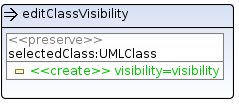
\includegraphics[width=0.40\textwidth]{pics/editClassVisibility.png}
  \caption{editClassVisibility}
  \label{editClassVisibility}
\end{figure}
%----------moveClass----------------------------------------
\op
{moveClass}
{moves a class from a package to another package}
{moveClass(Class selectedEObject, Package tgt)}
{The class which should be moved.}
{
\begin{itemize}
 \item tgt/tgt[moveClass]: the target package
\end{itemize}
}
{There is no class with the same name in the target context (see
\ref{subsec:checkOtherNames})}
{Only references will change.}
\begin{figure}[H]
  \centering
  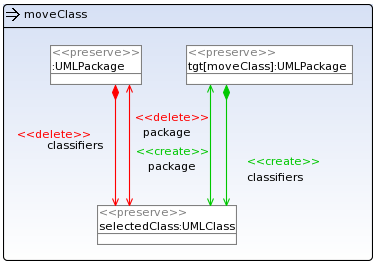
\includegraphics[width=0.65\textwidth]{pics/moveClass.png}
  \caption{moveClass}
  \label{moveClass}
\end{figure}

\newpage
\section{Interfaces}
%----------createInterface----------------------------------------
\op
{createInterface}
{creates a new interface}
{createInterface(Package selectedEObject, String nameValue, String idValue)}
{The package providing the container for the newly created interface.}
{
\begin{itemize}
 \item nameValue/newName: The name of the newly created interface
 \item idValue/newID: The id of the newly created interface
\end{itemize}
}
{There is no interface whose name equals the parameter-value of 'newName' (see
\ref{subsec:checkOtherNames})}
{Only the name and the id will be set via input data. Visibility will be set
with a default value as defined with the diagram editor in the image below.}
\begin{figure}[H]
  \centering
  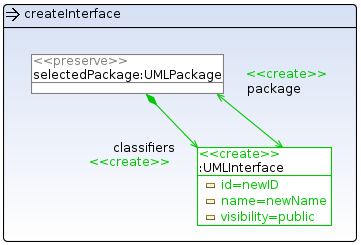
\includegraphics[width=0.65\textwidth]{pics/createInterface.png}
  \caption{createInterface}
  \label{createInterface}
\end{figure}
%----------deleteInterface----------------------------------------
\op
{deleteInterface}
{Deletes an interface}
{deleteInterface(Interface selectedEObject)}
{The interface which should be deleted} {-}
{-}
{For a better readability this is a simplified version of the
'deleteInterface'-transformation and will only cover cases where the
interfac has no containments and no references to other elements. Such a
complex transformation rule exits but won't be listed here.}
\begin{figure}[H]
  \centering
  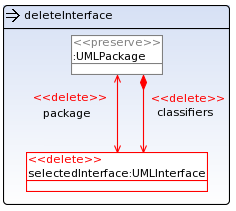
\includegraphics[width=0.4\textwidth]{pics/deleteInterface_emptyAndUnreferenced.png}
  \caption{deleteInterface}
  \label{deleteInterface}
\end{figure}

%----------editInterfaceName----------------------------------------
\op
{editInterfaceName}
{edits the name of an interface}
{editInterfaceName(Interface selectedEObject, String nameValue)}
{The interface whose name should be renamed.}
{
\begin{itemize}
 \item nameValue/newName: The new name
\end{itemize}
}
{There is no interface in the same package whose name equals the parameter-value of
'newName' (see
\ref{subsec:checkOtherNames})}
{The \textless\textless create\textgreater\textgreater  -symbol in the image
means that even if the attribute exists its value will be overwritten.
'newName' is the placeholder for the input name.}
\begin{figure}[H]
  \centering
  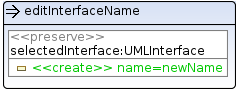
\includegraphics[width=0.4\textwidth]{pics/editInterfaceName.png}
  \caption{editInterfaceName}
  \label{editInterfaceName}
\end{figure}
%----------editInterfaceVisibility----------------------------------------
\op
{editInterfaceVisibility}
{edits the visibility of an interface}
{editInterfaceVisibility(Interface selectedEObject, Visibility visibilityValue)}
{The interface whose visibility should be edited.}
{
\begin{itemize}
 \item visibilityValue/visibility: The new visiblility
\end{itemize}
}
{-}
{The \textless\textless create\textgreater\textgreater  -symbol in the image
means that even if the attribute exists its value will be overwritten.
'visibility' is the placeholder for the input visibility value.}
\begin{figure}[H]
  \centering
  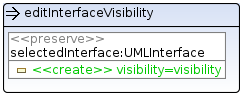
\includegraphics[width=0.4\textwidth]{pics/editInterfaceVisibility.png}
  \caption{editInterfaceVisibility}
  \label{editInterfaceVisibility}
\end{figure}
%----------moveInterface----------------------------------------
\op
{moveInterface}
{moves an interface from a package to another package}
{moveInterface(Interface selectedEObject, Package tgt)}
{The interface which should be moved.}
{
\begin{itemize}
 \item tgt/tgt[moveInterface]: the target package
\end{itemize}
}
{There is no interface with the same name in the target context (see
\ref{subsec:checkOtherNames})}
{Only references will change}
\begin{figure}[H]
  \centering
  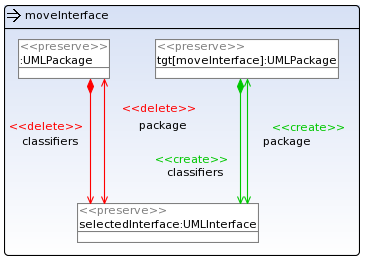
\includegraphics[width=0.65\textwidth]{pics/moveInterface.png}
  \caption{moveInterface}
  \label{moveInterface}
\end{figure}

\newpage
\section{Enumerations}
%----------createEnumeration----------------------------------------
\op
{createEnumeration}
{creates a new enumeration}
{createEnumeration(Package selectedEObject, String nameValue, String idValue)}
{The package providing the container for the newly created enumeration.}
{
\begin{itemize}
 \item nameValue/newName: The name of the newly created enumeration
 \item idValue/newID: The id of the newly created enumeration
\end{itemize}
}
{There is no enumeration whose name equals the parameter-value of 'newName' (see
\ref{subsec:checkOtherNames})}
{Only the name and the id will be set via input data. Visibility will be set
with a default value as defined with the diagram editor in the image below.}
\begin{figure}[H]
  \centering
  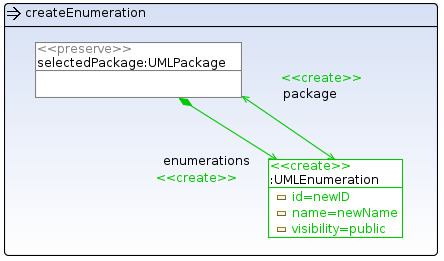
\includegraphics[width=0.65\textwidth]{pics/createEnumeration.png}
  \caption{createEnumeration}
  \label{createEnumeration}
\end{figure}
%----------deleteEnumeration----------------------------------------
\op
{deleteEnumeration}
{Deletes an enumeration}
{deleteEnumeration(Enumeration selectedEObject)}
{The enumeration which should be deleted}
{-}
{-}
{For a better readability this is a simplified version of the
'deleteEnumeration'-transformation and will only cover cases where the
enumeration has no containments and no references to other elements. Such a
complex transformation rule exits but won't be listed here.}
\begin{figure}[H]
  \centering
  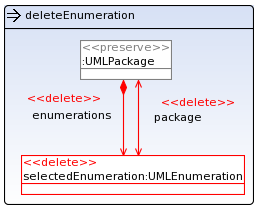
\includegraphics[width=0.4\textwidth]{pics/deleteEnumeration_emptyAndUnreferenced.png}
  \caption{deleteEnumeration}
  \label{deleteEnumeration}
\end{figure}
%----------editEnumerationName----------------------------------------
\op
{editEnumerationName}
{edits the name of an enumeration}
{editEnumerationName(Enumeration selectedEObject, String nameValue)}
{The enumeration whose name should be renamed.}
{
\begin{itemize}
 \item nameValue/newName: The new name
\end{itemize}
}
{There is no enumeration in the same package whose name equals the parameter-value of
'newName' (see
\ref{subsec:checkOtherNames})}
{The \textless\textless create\textgreater\textgreater  -symbol in the image
means that even if the attribute exists its value will be overwritten.
'newName' is the placeholder for the input name.}
\begin{figure}[H]
  \centering
  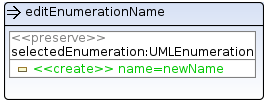
\includegraphics[width=0.4\textwidth]{pics/editEnumerationName.png}
  \caption{editEnumerationName}
  \label{editEnumerationName}
\end{figure}
%----------editEnumerationVisibility----------------------------------------
\op
{editEnumerationVisibility}
{edits the visibility of an enumeration}
{editEnumerationVisibility(Enumeration selectedEObject, Visibility visibilityValue)}
{The enumeration whose visibility should be edited.}
{
\begin{itemize}
 \item visibilityValue/visibility: The new visiblility
\end{itemize}
}
{-}
{The \textless\textless create\textgreater\textgreater  -symbol in the image
means that even if the attribute exists its value will be overwritten.
'visibility' is the placeholder for the input visibility value.}
\begin{figure}[H]
  \centering
  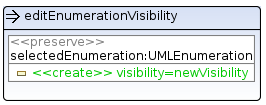
\includegraphics[width=0.4\textwidth]{pics/editEnumerationVisibility.png}
  \caption{editEnumerationVisibility}
  \label{editEnumerationVisibility}
\end{figure}
%----------moveEnumeration----------------------------------------
\op
{moveEnumeration}
{moves an enumeration from a package to another package}
{moveEnumeration(Enumeration selectedEObject, Package tgt)}
{The enumeration which should be moved.}
{
\begin{itemize}
 \item tgt/tgt[moveEnumeration]: the target package
\end{itemize}
}
{There is no enumeration with the same name in the target context (see
\ref{subsec:checkOtherNames})}
{Only references will change.}
\begin{figure}[H]
  \centering
  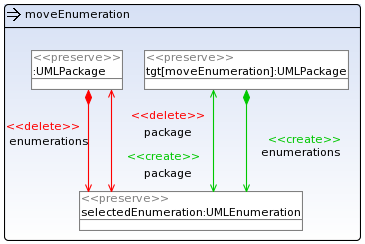
\includegraphics[width=0.65\textwidth]{pics/moveEnumeration.png}
  \caption{moveEnumeration}
  \label{moveEnumeration}
\end{figure}

\newpage
\section{Literals}
%----------createLiteral----------------------------------------
\op
{createLiteral}
{creates a new literal}
{createLiteral(Package selectedEObject, String nameValue)}
{The package providing the container for the newly created literal.}
{
\begin{itemize}
 \item nameValue/newName: The name of the newly created literal
 \item idValue/newID: The id of the newly created literal
\end{itemize}
}
{There is no literal whose name equals the parameter-value of 'newID' (see
\ref{subsec:checkOtherNames})}
{The name and the id will be set via input data.}
\begin{figure}[H]
  \centering
  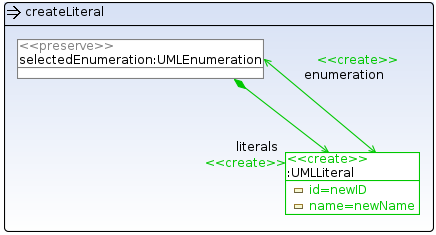
\includegraphics[width=0.65\textwidth]{pics/createLiteral.png}
  \caption{createLiteral}
  \label{createLiteral}
\end{figure}
%----------deleteLiteral----------------------------------------
\op
{deleteLiteral}
{Deletes a literal}
{deleteLiteral(Literal selectedEObject)}
{The literal which should be deleted}
{-}
{-}
{For a better readability this is a simplified version of the
'deleteLiteral'-transformation and will only cover cases where the
literal has no references to other elements. Such a
complex transformation rule exits but won't be listed here.}
\begin{figure}[H]
  \centering
  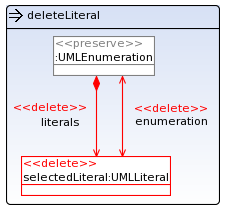
\includegraphics[width=0.4\textwidth]{pics/deleteLiteral_emptyAndUnreferenced.png}
  \caption{deleteLiteral}
  \label{deleteLiteral}
\end{figure}
%----------editLiteralName----------------------------------------
\op
{editLiteralName}
{edits the name of a literal}
{editLiteralName(Literal selectedEObject, String nameValue)}
{The literal whose name should be renamed.}
{
\begin{itemize}
 \item nameValue/newName: The new name
\end{itemize}
}
{There is no literal in the same package whose name equals the parameter-value of
'newName' (see
\ref{subsec:checkOtherNames})}
{The \textless\textless create\textgreater\textgreater  -symbol in the image
means that even if the attribute exists its value will be overwritten.
'newName' is the placeholder for the input name.}
\begin{figure}[H]
  \centering
  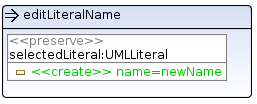
\includegraphics[width=0.4\textwidth]{pics/editLiteralName.png}
  \caption{editLiteralName}
  \label{editLiteralName}
\end{figure}
%----------moveLiteral----------------------------------------
\op
{moveLiteral}
{moves a literal from an enumeration to another}
{moveLiteral(Literal selectedEObject, Enumeration tgt)}
{The literal which should be moved.}
{
\begin{itemize}
 \item tgt/tgt[moveLiteral]: the target enumeration
\end{itemize}
}
{There is no literal with the same name in the target context (see
\ref{subsec:checkOtherNames})}
{Only references will change.}
\begin{figure}[H]
  \centering
  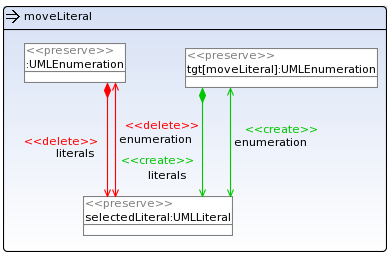
\includegraphics[width=0.65\textwidth]{pics/moveLiteral.png}
  \caption{moveLiteral}
  \label{moveLiteral}
\end{figure}

\newpage
\section{PrimitiveTypes}
%----------createPrimitiveType----------------------------------------
\op
{createPrimitiveType}
{creates a new primitiveType}
{createPrimitiveType(Package selectedEObject, String nameValue, String idValue)}
{The package providing the container for the newly created primitiveType.}
{
\begin{itemize}
 \item nameValue/newName: The name of the newly created primitiveType
 \item idValue/newID: The id of the newly created pimitiveType
\end{itemize}
}
{There is no primitiveType whose name equals the parameter-value of 'newName' (see
\ref{subsec:checkOtherNames})}
{The name and the id will be set via input data.}
\begin{figure}[H]
  \centering
  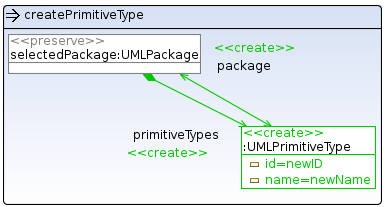
\includegraphics[width=0.65\textwidth]{pics/createPrimitiveType.png}
  \caption{createPrimitiveType}
  \label{createPrimitiveType}
\end{figure}
%----------deletePrimitiveType----------------------------------------
\op
{deletePrimitiveType}
{Deletes a primitiveType}
{deletePrimitiveType(PrimitiveType selectedEObject)}
{The primitiveType which should be deleted}
{-}
{-}
{For a better readability this is a simplified version of the
'deletePrimitiveType'-transformation and will only cover cases where the
primitiveType has no references to other elements. Such a
complex transformation rule exits but won't be listed here.}
\begin{figure}[H]
  \centering
  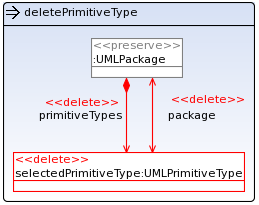
\includegraphics[width=0.4\textwidth]{pics/deletePrimitiveType_emptyAndUnreferenced.png}
  \caption{deletePrimitiveType}
  \label{deletePrimitiveType}
\end{figure}
%----------editPrimitiveTypeName----------------------------------------
\op
{editPrimitiveTypeName}
{edits the name of a primitiveType}
{editPrimitiveTypeName(PrimitiveType selectedEObject, String nameValue)}
{The primitiveType whose name should be renamed.}
{
\begin{itemize}
 \item nameValue/newName: The new name
\end{itemize}
}
{There is no primitiveType in the same package whose name equals the parameter-value of
'newName' (see \ref{subsec:checkOtherNames})}
{The \textless\textless create\textgreater\textgreater  -symbol in the image
means that even if the attribute exists its value will be overwritten.
'newName' is the placeholder for the input name.}
\begin{figure}[H]
  \centering
  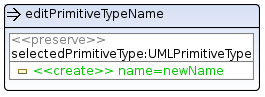
\includegraphics[width=0.4\textwidth]{pics/editPrimitiveTypeName.png}
  \caption{editPrimitiveTypeName}
  \label{editPrimitiveTypeName}
\end{figure}
%----------movePrimitiveType----------------------------------------
\op
{movePrimitiveType}
{moves a primitiveType from a package to another package}
{movePrimitiveType(PrimitiveType selectedEObject, Package tgt)}
{The primitiveType which should be moved.}
{
\begin{itemize}
 \item tgt/tgt[movePrimitiveType]: the target package
\end{itemize}
}
{There is no primitiveType with the same name in the target context (see
\ref{subsec:checkOtherNames})}
{Only references will change}
\begin{figure}[H]
  \centering
  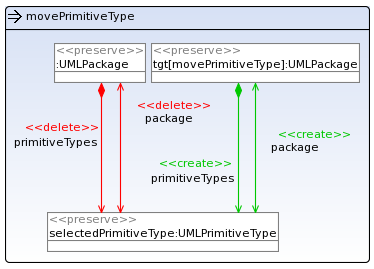
\includegraphics[width=0.65\textwidth]{pics/movePrimitiveType.png}
  \caption{movePrimitiveType}
  \label{movePrimitiveType}
\end{figure}

\newpage
\section{Stereotypes}
%----------createStereotype----------------------------------------
\op
{createStereotype}
{creates a new stereotype}
{createStereotype(Package selectedEObject, String nameValue)}
{The model providing the container for the newly created stereotype.}
{
\begin{itemize}
 \item nameValue/newName: The name of the newly created stereotype
 \item idValue/newID: The id of the newly created stereotype
\end{itemize}
}
{There is no stereotype whose name equals the parameter-value of 'newName' (see
\ref{subsec:checkOtherNames})}
{Only the name and the id will be set via input data.}
\begin{figure}[H]
  \centering
  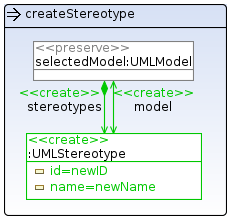
\includegraphics[width=0.4\textwidth]{pics/createStereotype.png}
  \caption{createStereotype}
  \label{createStereotype}
\end{figure}
%----------deleteStereotype----------------------------------------
\op
{deleteStereotype}
{Deletes a stereotype}
{deleteStereotype(Stereotype selectedEObject)}
{The stereotype which should be deleted}
{-}
{-}
{For a better readability this is a simplified version of the
'deleteStereotype'-transformation and will only cover cases where the stereotype
has no containments and no references to other elements. Such a complex
transformation rule exits but won't be listed here.}
\begin{figure}[H]
  \centering
  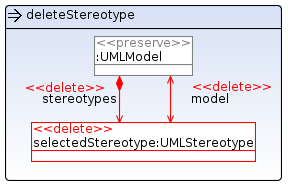
\includegraphics[width=0.4\textwidth]{pics/deleteStereotype_emptyAndUnreferenced.png}
  \caption{deleteStereotype}
  \label{deleteStereotype}
\end{figure}
%----------editStereotypeName----------------------------------------
\op
{editStereotypeName}
{edits the name of a stereotype}
{editStereotypeName(Stereotype selectedEObject, String nameValue)}
{The stereotype whose name should be renamed.}
{
\begin{itemize}
 \item nameValue/newName: The new name
\end{itemize}
}
{There is no stereotype in the same package whose name equals the parameter-value of
'newName' (see
\ref{subsec:checkOtherNames})}
{The \textless\textless create\textgreater\textgreater  -symbol in the image
means that even if the attribute exists its value will be overwritten.
'newName' is the placeholder for the input name.}
\begin{figure}[H]
  \centering
  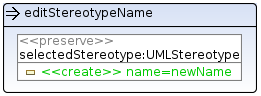
\includegraphics[width=0.4\textwidth]{pics/editStereotypeName.png}
  \caption{editStereotypeName}
  \label{editStereotypeName}
\end{figure}

\newpage
\section{Associations}
%----------createAssociationBetweenClasses----------------------------------------
\op
{createAssociationBetweenClasses}
{creates a new association between classes}
{createAssociationBetweenClasses(Package selectedEObject, String nameValue,
String idValue, String srcMultiplicity)} {The package providing the container
for the newly created association.} {
\begin{itemize}
 \item nameValue/newName: The name of the newly created association
 \item idValue/newID: The id of the newly created association
 \item srcValue/newSrcName: The name of the newly created source association end
 \item srcIdValue/newSrcID: The id of the newly created source association end
 \item srcMultiplicity/newMultiplicity: The multiplicity of the newly created
 source association end
 \item tgtValue/newTgtName: The name of the newly created target association end
 \item tgtIdValue/newTgtID: The id of the newly created target association end
 \item tgtMultiplicity/newMultiplicity: The multiplicity of the newly created
 target association end
\end{itemize}
}
{The 'newSrcName' and 'newTgtName' must differ (see
\ref{subsec:checkOtherNames})}
{This rule firstly creates an association under the propagated package with
input data for id and name. Secondly it will create association ends with input data for id, name and
multiplicity (isNavigatable, kind and isOrdered will recieve default
values). Afterwards it will append them to the association created beforehand
via references (association and associationEnds). Lastly the association
ends will either get a reference (target) to an input class.
\\Note that the reference from a class and from the selected association point to
the same unknown package. This will make sure that there won't be created
associations between classes of different packages.}
\begin{figure}[H]
  \centering
  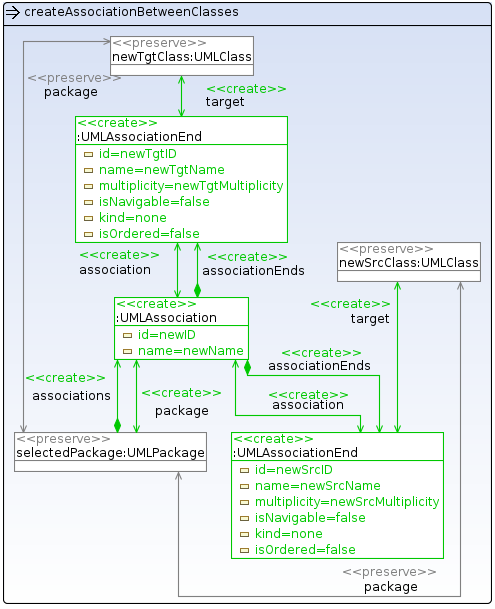
\includegraphics[width=0.8\textwidth]{pics/createAssociationBetweenClasses.png}
  \caption{createAssociationBetweenClasses}
  \label{createAssociationBetweenClasses}
\end{figure}
%----------createAssociationBetweenInterfaces----------------------------------------
\op
{createAssociationBetweenInterfaces}
{creates a new association between interfaces}
{createAssociationBetweenInterfaces(Package selectedEObject, String nameValue,
String idValue, String srcMultiplicity)} {The package providing the container
for the newly created association.} {
\begin{itemize}
 \item nameValue/newName: The name of the newly created association
 \item idValue/newID: The id of the newly created association
 \item srcValue/newSrcName: The name of the newly created source association end
 \item srcIdValue/newSrcID: The id of the newly created source association end
 \item srcMultiplicity/newMultiplicity: The multiplicity of the newly created
 source association end
 \item tgtValue/newTgtName: The name of the newly created target association end
 \item tgtIdValue/newTgtID: The id of the newly created target association end
 \item tgtMultiplicity/newMultiplicity: The multiplicity of the newly created
 target association end
\end{itemize}
}
{The 'newSrcName' and 'newTgtName' must differ (see
\ref{subsec:checkOtherNames})}
{This rule firstly creates an association under the propagated package with
input data for id and name. Secondly it will create association ends with input data for id, name and
multiplicity (isNavigatable, kind and isOrdered will recieve default
values). Afterwards it will append them to the association created beforehand
via references (association and associationEnds). Lastly the association
ends will either get a reference (target) to an input interface.
\\Note that the reference from an interface and from the selected association
point to the same unknown package. This will make sure that there won't be created
associations between interfaces of different packages.}
\begin{figure}[H]
  \centering
  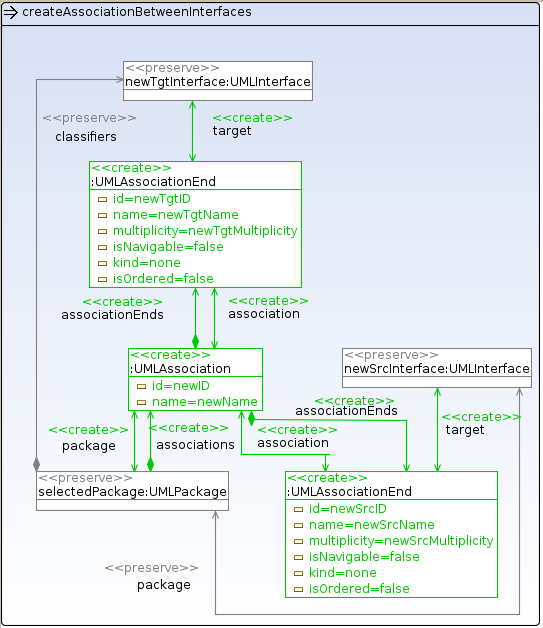
\includegraphics[width=0.8\textwidth]{pics/createAssociationBetweenInterfaces.png}
  \caption{createAssociationBetweenInterfaces}
  \label{createAssociationBetweenInterfaces}
\end{figure}
%----------deleteAssociation----------------------------------------
\op
{deleteAssociation}
{Deletes an association}
{deleteAssociation(Association selectedEObject)}
{The association which should be deleted including all its containments and all
its references}
{-}
{-}
{For this transformation three rules are needed. The first two will be used to
delete the target reference of an association end depending on the type of
the target. The third rule will delete the selected association from its
container package.
\\In the second picture you can find the TransformationUnits. It contains a
Sequential 'mainUnit' which will firstly run the Counted Unit
'LOOP\_deleteAssociationEndIsClass'. After there is no associaton end under the
selected association left which points to a class, the next Counted Unit
'LOOP\_deleteAssociationEndIsInterface' will be run. Both Counted Units behave
similarily. When there are no available association ends left, the
deleteAssociation-Rule will be called.}
\begin{figure}[H]
  \advance\leftskip-1.5cm
  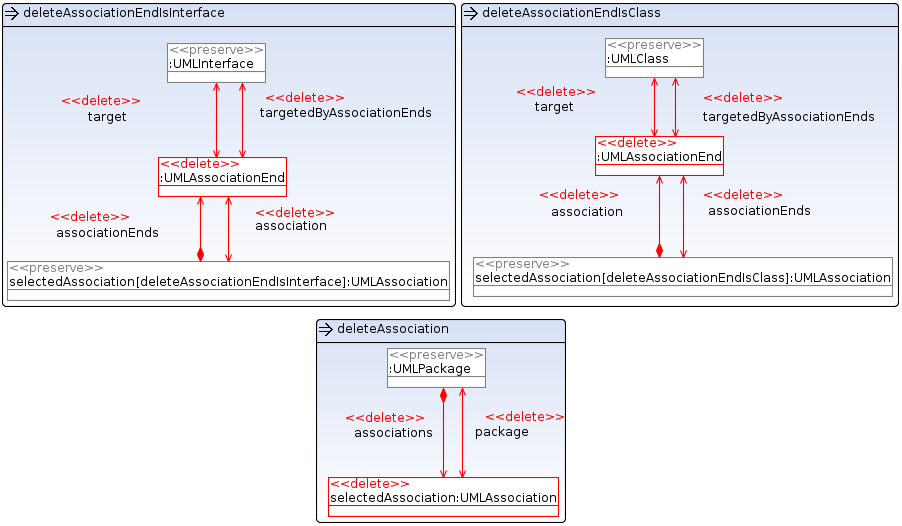
\includegraphics[width=1.2\textwidth]{pics/deleteAssociation.png}
  \caption{deleteAssociation}
  \label{deleteAssociation}
\end{figure}
\begin{figure}[H]
  \advance\leftskip-1.5cm
  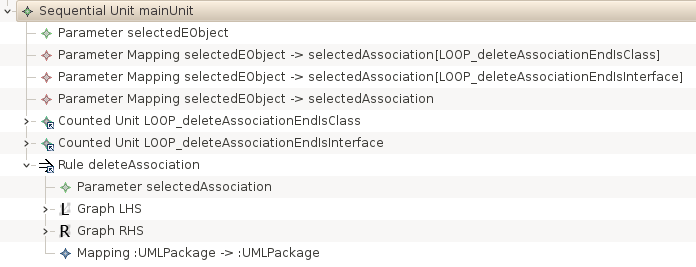
\includegraphics[width=1.2\textwidth]{pics/deleteAssociation_TreeView.png}
  \caption{deleteAssociation(UnitView)}
  \label{deleteAssociation(UnitView)}
\end{figure}
%----------editAssociationName----------------------------------------
\op
{editAssociationName}
{edits the name of an association}
{editAssociationName(Association selectedEObject, String nameValue)}
{The association whose name should be renamed.}
{
\begin{itemize}
 \item nameValue/newName: The new name
\end{itemize}
}
{-}
{The \textless\textless create\textgreater\textgreater  -symbol in the image
means that even if the attribute exists its value will be overwritten.
'newName' is the placeholder for the input name.}
\begin{figure}[H]
  \centering
  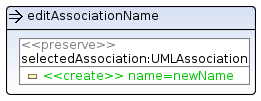
\includegraphics[width=0.45\textwidth]{pics/editAssociationName.png}
  \caption{editAssociationName}
  \label{editAssociationName}
\end{figure}

\newpage
\section{AssociationClasses}
Since the AssociationClass-Transformations are build the same like the
Association-Transformations with the only difference that the selectedEObject
of the edit- and delete-Transformations is an AssociationClass instead of an
Association they won't be covered here.

\newpage
\section{AssociationEnds}
%----------createAssociationEndIsClass----------------------------------------
\op
{createAssociationEndIsClass}
{Creates a new association end under the selected association and links it to a
class that lies in the same package as the association}
{createAssociationEndIsClass(Association
selectedEObject, String nameValue, String idValue, String srcMultiplicity)} {The
association providing the container for the newly created association end.} {
\begin{itemize}
 \item nameValue/newName: The name of the newly created association end
 \item idValue/newID: The id of the newly created association end
 \item srcMultiplicity/newMultiplicity: The multiplicity of the newly created
 source association end
\end{itemize}
}
{There mustn't be an association end under the selected association with the
same name like in 'newName' (see
\ref{subsec:checkOtherNames})}
{Only the name, id and multiplicity will be set via input data. isNavigable,
kind and isOrdered will be set with a default value as defined with the diagram
editor in the image below.
Note that the reference from a class and from the selected association point to
the same unknown package. This will make sure that there won't be created
associations between classes of different packages.}
\begin{figure}[H]
  \centering
  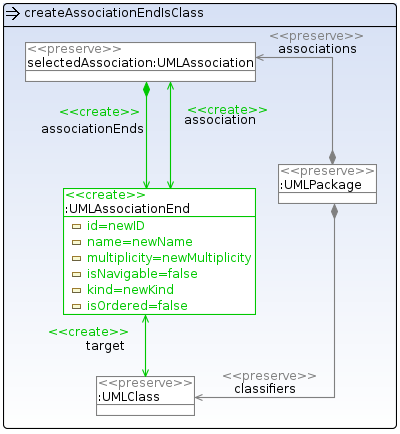
\includegraphics[width=0.65\textwidth]{pics/createAssociationEndIsClass.png}
  \caption{createAssociationEndIsClass}
  \label{createAssociationEndIsClass}
\end{figure}
%----------createAssociationEndIsInterface----------------------------------------
\op
{createAssociationEndIsInterface}
{Creates a new association end under the selected association and links it to an
interface that lies in the same package as the association}
{createAssociationEndIsInterface(Association
selectedEObject, String nameValue, String idValue, String srcMultiplicity)} {The
association providing the container for the newly created association end.} {
\begin{itemize}
 \item nameValue/newName: The name of the newly created association end
 \item idValue/newID: The id of the newly created association end
 \item srcMultiplicity/newMultiplicity: The multiplicity of the newly created
 source association end
\end{itemize}
}
{There mustn't be an association end under the selected association with the
same name like in 'newName' (see
\ref{subsec:checkOtherNames})}
{Only the name, id and multiplicity will be set via input data. isNavigable,
kind and isOrdered will be set with a default value as defined with the diagram
editor in the image below.
Note that the reference from an interface and from the selected association
point to the same unknown package. This will make sure that there won't be created
associations between interfaces of different packages.}
\begin{figure}[H]
  \centering
  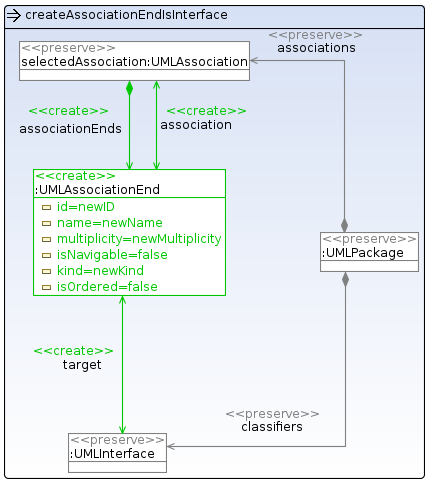
\includegraphics[width=0.65\textwidth]{pics/createAssociationEndIsInterface.png}
  \caption{createAssociationEndIsInterface}
  \label{createAssociationEndIsInterface}
\end{figure}
%----------deleteAssociationEnd----------------------------------------
\op
{deleteAssociationEnd}
{Deletes an association end and the reference to its actuall target, but not
the target itself}
{deleteAssociationEnd(AssociationEnd selectedEObject)}
{The association end which should be deleted including its reference}
{-}
{-}
{This transformation is designed with three rules. The first two rules will
delete an association end depending on which type it points to. The third one
will simply do nothing but is still required in the TransformationUnits.
\\\\You can see that the 'mainUnit' is a Conditional Unit this time. It will try to
run the rule 'deleteAssociationEndIsClass' and in case it will match this
means that the modification has worked and there is nothing left to do (that's
why a 'doNothing-Rule' is following in the 'Then'-part). Otherwise, if our
selected association end does not point to a class, we assume that it can only point to
an interface and therefore 'deleteAssociationEndIsInterface' will be called.
}
\begin{figure}[H]
  \centering
  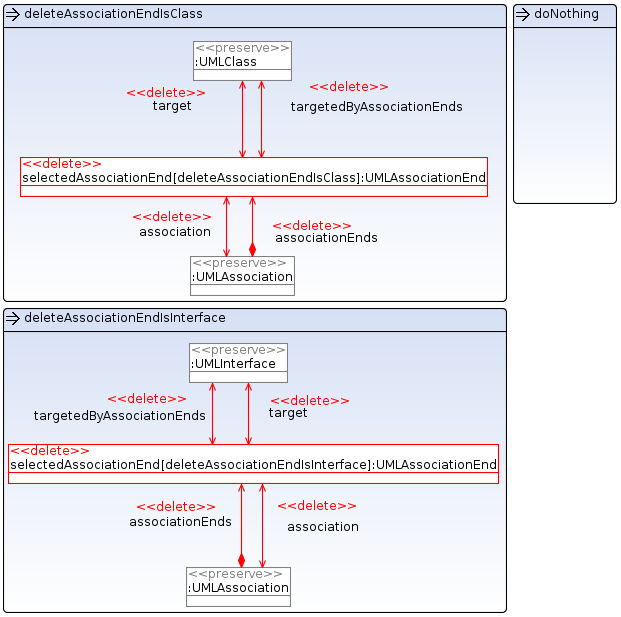
\includegraphics[width=0.8\textwidth]{pics/deleteAssociationEnd.png}
  \caption{deleteAssociationEnd}
  \label{deleteAssociationEnd}
\end{figure}
\begin{figure}[H]
  \centering
  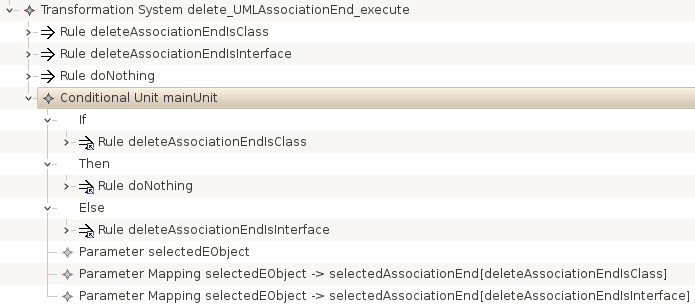
\includegraphics[width=1.0\textwidth]{pics/deleteAssociationEnd_TreeView.png}
  \caption{deleteAssociationEnd(UnitView)}
  \label{deleteAssociationEnd(UnitView)}
\end{figure}
%----------editAssociationEndFromClassToClass----------------------------------------
\op
{editAssociationEndFromClassToClass}
{Edits the target of an association end to another class}
{editAssociationEndFromClassToClass(AssociationEnd selectedEObject, Class
tgt)}
{The association end whose target should be changed}
{
\begin{itemize}
 \item tgt/targetClass: The new class
\end{itemize}
}
{-}
{Only references will change.}
\begin{figure}[H]
  \centering
  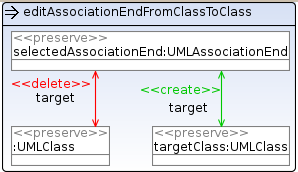
\includegraphics[width=0.4\textwidth]{pics/editAssociationEndFromClassToClass.png}
  \caption{editAssociationEndFromClassToClass}
  \label{editAssociationEndFromClassToClass}
\end{figure}
%----------editAssociationEndFromClassToInterface----------------------------------------
\op
{editAssociationEndFromClassToInterface}
{Edits the target of an association end from a class to an interface}
{editAssociationEndFromClassToInterface(AssociationEnd selectedEObject,
Interface tgt)}
{The association end whose target should be changed}
{
\begin{itemize}
 \item tgt/targetInterface: The new interface
\end{itemize}
}
{-}
{Only references will change.}
\begin{figure}[H]
  \centering
  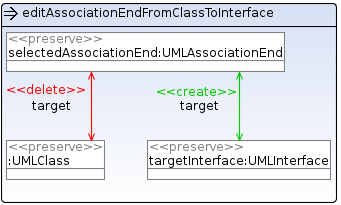
\includegraphics[width=0.45\textwidth]{pics/editAssociationEndFromClassToInterface.png}
  \caption{editAssociationEndFromClassToInterface}
  \label{editAssociationEndFromClassToInterface}
\end{figure}
%----------editAssociationEndFromInterfaceToClass----------------------------------------
\op
{editAssociationEndFromInterfaceToClass}
{Edits the target of an association end from an interface to a class}
{editAssociationEndFromInterfaceToClass(AssociationEnd selectedEObject,
Class tgt)}
{The association end whose target should be changed}
{
\begin{itemize}
 \item tgt/targetClass: The new class
\end{itemize}
}
{-}
{Only references will change.}
\begin{figure}[H]
  \centering
  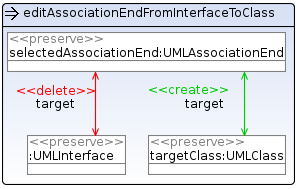
\includegraphics[width=0.4\textwidth]{pics/editAssociationEndFromInterfaceToClass.png}
  \caption{editAssociationEndFromInterfaceToClass}
  \label{editAssociationEndFromInterfaceToClass}
\end{figure}
%----------editAssociationEndFromInterfaceToInterface----------------------------------------
\op
{editAssociationEndFromInterfaceToInterface}
{Edits the target of an association end to another interface}
{editAssociationEndFromInterfaceToInterface(AssociationEnd selectedEObject,
Interface tgt)}
{The association end whose target should be changed}
{
\begin{itemize}
 \item tgt/targetInterface: The new interface
\end{itemize}
}
{-}
{Only references will change.}
\begin{figure}[H]
  \centering
  \includegraphics[width=0.45\textwidth]{pics/editAssociationEndFromInterfaceToInterface.png}
  \caption{editAssociationEndFromInterfaceToInterface}
  \label{editAssociationEndFromInterfaceToInterface}
\end{figure}
%----------editAssociationEndIsNavigatable----------------------------------------
\op
{editAssociationEndIsNavigatable}
{Edits the isNavigatable-value of an association end}
{editAssociationEndIsNavigatable(AssociationEnd selectedEObject, boolean
booleanValue)}
{The association end whose isNavigatable-value should be edited.}
{
\begin{itemize}
 \item booleanValue/bool: The new isNavigatable-value
\end{itemize}
}
{-}
{The \textless\textless create\textgreater\textgreater  -symbol in the image
means that even if the attribute exists its value will be overwritten.
'bool' is the placeholder for the input bool value.}
\begin{figure}[H]
  \centering
  \includegraphics[width=0.45\textwidth]{pics/editAssociationEndIsNavigatable.png}
  \caption{editAssociationEndIsNavigatable}
  \label{editAssociationEndIsNavigatable}
\end{figure}
%----------editAssociationEndIsOrdered----------------------------------------
\op
{editAssociationEndIsOrdered}
{Edits the isOrdered-value of an association end}
{editAssociationEndIsOrdered(AssociationEnd selectedEObject, boolean
booleanValue)}
{The association end whose isOrdered-value should be edited.}
{
\begin{itemize}
 \item booleanValue/bool: The new isOrdered-value
\end{itemize}
}
{-}
{The \textless\textless create\textgreater\textgreater  -symbol in the image
means that even if the attribute exists its value will be overwritten.
'bool' is the placeholder for the input bool value.}
\begin{figure}[H]
  \centering
  \includegraphics[width=0.4\textwidth]{pics/editAssociationEndIsOrdered.png}
  \caption{editAssociationEndIsOrdered}
  \label{editAssociationEndIsOrdered}
\end{figure}
%----------editAssociationEndName----------------------------------------
\op
{editAssociationEndName}
{Edits the name of an association end}
{editAssociationEndName(AssociationEnd selectedEObject, String nameValue)}
{The class whose name should be renamed.}
{
\begin{itemize}
 \item nameValue/newName: The new name
\end{itemize}
}
{There is no association end under the same association whose name equals the
parameter-value of 'newName' (see
\ref{subsec:checkOtherNames})}
{The \textless\textless create\textgreater\textgreater  -symbol in the image
means that even if the attribute exists its value will be overwritten.
'newName' is the placeholder for the input name.}
\begin{figure}[H]
  \centering
  \includegraphics[width=0.4\textwidth]{pics/editAssociationEndName.png}
  \caption{editAssociationEndName}
  \label{editAssociationEndName}
\end{figure}
%----------editAssociationEndKind----------------------------------------
\op
{editAssociationEndKind}
{Edits the kind (none, shared or composit) of an association end}
{editAssociationEndKind(AssociationEnd selectedEObject, Kind kindValue)}
{The class whose name should be renamed.}
{
\begin{itemize}
 \item kindValue/newKind: The new kind
\end{itemize}
}
{The opposit ending mustn't also be composit if the new kind is composit
(see
\ref{subsec:checkOppositeAggregationKind})}
{The \textless\textless create\textgreater\textgreater  -symbol in the image
means that even if the attribute exists its value will be overwritten.
'newKind' is the placeholder for the input kind value.}
\begin{figure}[H]
  \centering
  \includegraphics[width=0.45\textwidth]{pics/editAssociationEndKind.png}
  \caption{editAssociationEndKind}
  \label{editAssociationEndKind}
\end{figure}
%----------editAssociationEndMultiplicity----------------------------------------
\op
{editAssociationEndMultiplicity}
{Edits the multiplicity of an association end}
{editAssociationEndMultiplicity(AssociationEnd selectedEObject, String
srcMultiplicity)}
{The class whose name should be renamed.}
{
\begin{itemize}
 \item srcMultiplicity/newMultiplicity: The new multiplicity
\end{itemize}
}
{-}
{The \textless\textless create\textgreater\textgreater  -symbol in the image
means that even if the attribute exists its value will be overwritten.
'newMultiplicity' is the placeholder for the input multiplicity value.}
\begin{figure}[H]
  \centering
  \includegraphics[width=0.45\textwidth]{pics/editAssociationEndMultiplicity.png}
  \caption{editAssociationEndMultiplicity}
  \label{editAssociationEndMultiplicity}
\end{figure}

\newpage
\section{Generalizations}
%----------createGeneralizationBetweenAssociations----------------------------------------
\op
{createGeneralizationBetweenAssociations}
{Creates a new generalization relationship between two associations}
{createGeneralizationBetweenAssociations(Association selectedEObject,
Association tgt)}
{The association which will become the general element}
{
\begin{itemize}
 \item tgt/targetAssociation: the association which will become the special
 element and inherit from the general element
\end{itemize}
}
{The new generalization relationship must not create an inheritance-cycle (see
\ref{subsec:checkInheritanceCycle})}
{A generalization and references to the input selected association
(the parent) and the target association (the child) are created.} \begin{figure}[H]
  \centering
  \includegraphics[width=0.8\textwidth]{pics/createGeneralizationBetweenAssociations.png}
  \caption{createGeneralizationBetweenAssociations}
  \label{createGeneralizationBetweenAssociations}
\end{figure}
%----------createGeneralizationBetweenClasses----------------------------------------
\op
{createGeneralizationBetweenClasses}
{Creates a new generalization relationship between classes}
{createGeneralizationBetweenClasses(Class selectedEObject,
Class tgt)}
{The class which will become the general element}
{
\begin{itemize}
 \item tgt/targetClass: the class which will become the special
 element and inherit from the general element
\end{itemize}
}
{The new generalization relationship must not create an inheritance-cycle (see
\ref{subsec:checkInheritanceCycle})}
{A generalization and references to the input selected class
(the parent) and the target class (the child) are created.}
\begin{figure}[H]
  \centering
  \includegraphics[width=0.8\textwidth]{pics/createGeneralizationBetweenClasses.png}
  \caption{createGeneralizationBetweenClasses}
  \label{createGeneralizationBetweenClasses}
\end{figure}
%----------createGeneralizationBetweenInterfacees----------------------------------------
\op
{createGeneralizationBetweenInterfaces}
{Creates a new generalization relationship between interfaces}
{createGeneralizationBetweenInterfacees(Interface selectedEObject,
Interface tgt)}
{The interface which will become the general element}
{
\begin{itemize}
 \item tgt/targetInterface: the interface which will become the special
 element and inherit from the general element
\end{itemize}
}
{The new generalization relationship must not create an inheritance-cycle (see
\ref{subsec:checkInheritanceCycle})}
{A generalization and references to the input selected interface
(the parent) and the target interface (the child) are created.}
\begin{figure}[H]
  \centering
  \includegraphics[width=0.8\textwidth]{pics/createGeneralizationBetweenInterfaces.png}
  \caption{createGeneralizationBetweenInterfaces}
  \label{createGeneralizationBetweenInterfaces}
\end{figure}
%----------deleteGeneralizationBetweenAssociations----------------------------------------
\op
{deleteGeneralizationBetweenAssociations}
{Deletes a generalization between associations}
{deleteGeneralizationBetweenAssociations(Generalization selectedEObject)}
{The generalization which should be deleted}
{-}
{-}
{First the references from the associations to the generalization are deleted
and then the selected generalization itself.} \begin{figure}[H]
  \centering
  \includegraphics[width=0.8\textwidth]{pics/deleteGeneralizationBetweenAssociations.png}
  \caption{deleteGeneralizationBetweenAssociations}
  \label{deleteGeneralizationBetweenAssociations}
\end{figure}
%----------deleteGeneralizationBetweenAssociations----------------------------------------
\op
{deleteGeneralizationBetweenClasses}
{Deletes a generalization between classes}
{deleteGeneralizationBetweenClasses(Generalization selectedEObject)}
{The generalization which should be deleted}
{-}
{-}
{First the references from the classes to the generalization are deleted
and then the selected generalization itself.}
\begin{figure}[H]
  \centering
  \includegraphics[width=0.8\textwidth]{pics/deleteGeneralizationBetweenClasses.png}
  \caption{deleteGeneralizationBetweenClasses}
  \label{deleteGeneralizationBetweenClasses}
\end{figure}
%----------deleteGeneralizationBetweenInterfaces----------------------------------------
\op
{deleteGeneralizationBetweenInterfaces}
{Deletes a generalization between interfaces}
{deleteGeneralizationBetweenInterfaces(Generalization selectedEObject)}
{The generalization which should be deleted}
{-}
{-}
{First the references from the interfaces to the generalization are deleted
and then the selected generalization itself.}
\begin{figure}[H]
  \centering
  \includegraphics[width=0.8\textwidth]{pics/deleteGeneralizationBetweenInterfaces.png}
  \caption{deleteGeneralizationBetweenInterfaces}
  \label{deleteGeneralizationBetweenInterfaces}
\end{figure}
%----------editGeneralizationGeneralElementFromAssociationToAssociation----------------------------------------
\op
{editGeneralizationGeneralElementFromAssociationToAssociation}
{Replaces the general element of a generalization from an association by
another}
{editGeneralizationGeneralElementFromAssociationToAssociation(Generalization
selectedEObject, Association src, Association tgt)}
{The generalization whose general element should be changed.} {
\begin{itemize}
 \item src/oldAssociation: The old association as general element
 \item tgt/newAssociation: The new association as general element
\end{itemize}
}
{The new generalization relationship must not create an inheritance-cycle (see
\ref{subsec:checkInheritanceCycle})}
{Only references change.}
\begin{figure}[H]
  \centering
  \includegraphics[width=1.0\textwidth]{pics/editGeneralizationGeneralElementFromAssociationToAssociation.png}
  \caption{editGeneralizationGeneralElementFromAssociationToAssociation}
  \label{editGeneralizationGeneralElementFromAssociationToAssociation}
\end{figure}
%----------editGeneralizationGeneralElementFromClassToClass----------------------------------------
\op
{editGeneralizationGeneralElementFromClassToClass}
{Replaces the general element of a generalization from an class by
another}
{editGeneralizationGeneralElementFromClassToClass(Generalization
selectedEObject, Class src, Class tgt)}
{The generalization whose general element should be changed.} {
\begin{itemize}
 \item src/oldClass: The old class as general element
 \item tgt/newClass: The new class as general element
\end{itemize}
}
{The new generalization relationship must not create an inheritance-cycle (see
\ref{subsec:checkInheritanceCycle})}
{Only references change.}
\begin{figure}[H]
  \centering
  \includegraphics[width=1.0\textwidth]{pics/editGeneralizationGeneralElementFromClassToClass.png}
  \caption{editGeneralizationGeneralElementFromClassToClass}
  \label{editGeneralizationGeneralElementFromClassToClass}
\end{figure}
%----------editGeneralizationGeneralElementFromInterfaceToInterface----------------------------------------
\op
{editGeneralizationGeneralElementFromInterfaceToInterface}
{Replaces the general element of a generalization from an interface by
another}
{editGeneralizationGeneralElementFromInterfaceToInterface(Generalization
selectedEObject, Interface src, Interface tgt)}
{The generalization whose general element should be changed.} {
\begin{itemize}
 \item src/oldInterface: The old interface as general element
 \item tgt/newInterface: The new interface as general element
\end{itemize}
}
{The new generalization relationship must not create an inheritance-cycle (see
\ref{subsec:checkInheritanceCycle})}
{Only references change.}
\begin{figure}[H]
  \centering
  \includegraphics[width=1.0\textwidth]{pics/editGeneralizationGeneralElementFromInterfaceToInterface.png}
  \caption{editGeneralizationGeneralElementFromInterfaceToInterface}
  \label{editGeneralizationGeneralElementFromInterfaceToInterface}
\end{figure}
%----------editGeneralizationSpecialElementFromInterfaceToInterface----------------------------------------
\op
{editGeneralizationSpecialElementFromInterfaceToInterface}
{Edits the special element of a specialization from an interface to
another}
{editGeneralizationSpecialElementFromInterfaceToInterface(Generalization
selectedEObject, Interface src, Interface tgt)}
{The specialization whose special element should be changed.} {
\begin{itemize}
 \item src/oldInterface: The old interface as special element
 \item tgt/newInterface: The new interface as special element
\end{itemize}
}
{The new generalization relationship must not create an inheritance-cycle (see
\ref{subsec:checkInheritanceCycle})}
{Only references change.}
\begin{figure}[H]
  \centering
  \includegraphics[width=1.0\textwidth]{pics/editGeneralizationSpecialElementFromInterfaceToInterface.png}
  \caption{editGeneralizationSpecialElementFromInterfaceToInterface}
  \label{editGeneralizationSpecialElementFromInterfaceToInterface}
\end{figure}
%----------editGeneralizationSpecialElementFromClassToClass----------------------------------------
\op
{editGeneralizationSpecialElementFromClassToClass}
{Edits the special element of a specialization from an class to
another}
{editGeneralizationSpecialElementFromClassToClass(Generalization
selectedEObject, Class src, Class tgt)}
{The specialization whose special element should be changed.} {
\begin{itemize}
 \item src/oldClass: The old class as special element
 \item tgt/newClass: The new class as special element
\end{itemize}
}
{The new generalization relationship must not create an inheritance-cycle (see
\ref{subsec:checkInheritanceCycle})}
{Only references change.}
\begin{figure}[H]
  \centering
  \includegraphics[width=1.0\textwidth]{pics/editGeneralizationSpecialElementFromClassToClass.png}
  \caption{editGeneralizationSpecialElementFromClassToClass}
  \label{editGeneralizationSpecialElementFromClassToClass}
\end{figure}
%----------editGeneralizationSpecialElementFromAssociationToAssociation----------------------------------------
\op
{editGeneralizationSpecialElementFromAssociationToAssociation}
{Edits the special element of a specialization from an association to
another}
{editGeneralizationSpecialElementFromAssociationToAssociation(Generalization
selectedEObject, Association src, Association tgt)}
{The specialization whose special element should be changed.} {
\begin{itemize}
 \item src/oldAssociation: The old association as special element
 \item tgt/newAssociation: The new association as special element
\end{itemize}
}
{The new generalization relationship must not create an inheritance-cycle (see
\ref{subsec:checkInheritanceCycle})}
{Only references change.}
\begin{figure}[H]
  \centering
  \includegraphics[width=1.0\textwidth]{pics/editGeneralizationSpecialElementFromAssociationToAssociation.png}
  \caption{editGeneralizationSpecialElementFromAssociationToAssociation}
  \label{editGeneralizationSpecialElementFromAssociationToAssociation}
\end{figure}


\newpage
\section{Operations}
%----------createOperationInClass----------------------------------------
\op
{createOperationInClass}
{creates a new operation in a class}
{createOperationInClass(Class selectedEObject, String nameValue, Class typeValue)}
{The class providing the container for the newly created operation.} {
\begin{itemize}
 \item nameValue/newName: The name of the newly created operation
 \item idValue/newID: The id of the newly created operation
 \item typeValue/newType: The type of the newly created operation
\end{itemize}
}
{There is no operation in the same context whose name equals the parameter-value
of 'newName' (see
\ref{subsec:checkOtherNames})}
{Only the name and the id will be set via input data. Visibility, isAbstract adn
isStatic will be set with a default value as defined with the diagram editor in
the image below. The 'newType' input data is a concrete propagated class.}
\begin{figure}[H]
  \centering
  \includegraphics[width=0.45\textwidth]{pics/createOperationInClass.png}
  \caption{createOperationInClass}
  \label{createOperationInClass}
\end{figure}
%----------createOperationInInterface----------------------------------------
\op
{createOperationInInterface}
{creates a new operation in an interface}
{createOperationInInterface(Interface selectedEObject, String nameValue, Class typeValue)}
{The interface providing the container for the newly created
operation.} {
\begin{itemize}
 \item nameValue/newName: The name of the newly created operation
 \item idValue/newID: The id of the newly created operation
 \item typeValue/newType: The type of the newly created operation
\end{itemize}
}
{There is no operation in the same context whose name equals the parameter-value
of 'newName' (see
\ref{subsec:checkOtherNames})}
{Only the name and the id will be set via input data. Visibility, isAbstract adn
isStatic will be set with a default value as defined with the diagram editor in
the image below. The 'newType' input data is a concrete propagated interface.}
\begin{figure}[H]
  \centering
  \includegraphics[width=0.45\textwidth]{pics/createOperationInInterface.png}
  \caption{createOperationInInterface}
  \label{createOperationInInterface}
\end{figure}
%----------deleteOperation----------------------------------------
\op
{deleteOperation}
{Deletes an operation}
{deleteOperation(Operation selectedEObject)}
{The operation which should be deleted} {-}
{-}
{For a better readability this is a simplified version of the
'deleteOperation'-transformation and will only cover cases where the operation
has no containments and no references to other elements. Such a complex
transformation rule exits but won't be listed here.
\\\\In this simplified version we have three rules. One that checks if the
container of the operation is a model and the other rules that deletes the
operation depending on the found container type. In the following image of the
units you can see the case distinction done with a Conditional Unit. We assume
the container is an interface if not a class.}
\begin{figure}[H]
\advance\leftskip-1.5cm
  \includegraphics[width=1.2\textwidth]{pics/deleteOperation_emptyAndUnreferenced.png}
  \caption{deleteOperation}
  \label{deleteOperation}
\end{figure}

\begin{figure}[H]
  \centering
  \includegraphics[width=1.0\textwidth]{pics/deleteOperation_emptyAndUnreferenced_TreeView.png}
  \caption{deleteOperation(UnitView)}
  \label{deleteOperation(UnitView)}
\end{figure}
%----------editOperationName----------------------------------------
\op
{editOperationName}
{edits the name of an operation}
{editOperationName(Operation selectedEObject, String nameValue)}
{The operation whose name should be renamed.}
{
\begin{itemize}
 \item nameValue/newName: The new name
\end{itemize}
}
{There is no operation in the same class whose name equals the parameter-value of
'newName' (see
\ref{subsec:checkOtherNames})}
{The \textless\textless create\textgreater\textgreater  -symbol in the image
means that even if the attribute exists its value will be overwritten.
'someName' is the placeholder for the input name.}
\begin{figure}[H]
  \centering
  \includegraphics[width=0.4\textwidth]{pics/editOperationName.png}
  \caption{editOperationName}
  \label{editOperationName}
\end{figure}
%----------editOperationIsAbstract----------------------------------------
\op
{editOperationIsAbstract}
{edits the isAbstract-value of an operation}
{editOperationIsAbstract(Operation selectedEObject, boolean booleanValue)}
{The operation whose isAbstract-value should be edited.}
{
\begin{itemize}
 \item booleanValue/bool: The new isAbstract-value
\end{itemize}
}
{The \textless\textless create\textgreater\textgreater  -symbol in the image
means that even if the attribute exists its value will be overwritten.
'bool' is the placeholder for the input boolean value.}
{safsdfsd}
\begin{figure}[H]
  \centering
  \includegraphics[width=0.4\textwidth]{pics/editOperationIsAbstract.png}
  \caption{editOperationIsAbstract}
  \label{editOperationIsAbstract}
\end{figure}
%----------editOperationIsStatic----------------------------------------
\op
{editOperationIsStatic}
{edits the isStatic-value of an operation}
{editOperationIsStatic(Operation selectedEObject, boolean booleanValue)}
{The operation whose isStatic-value should be edited.}
{
\begin{itemize}
 \item booleanValue/bool: The new isStatic-value
\end{itemize}
}
{-}
{The \textless\textless create\textgreater\textgreater  -symbol in the image
means that even if the attribute exists its value will be overwritten.
'bool' is the placeholder for the input boolean value.}
\begin{figure}[H]
  \centering
  \includegraphics[width=0.4\textwidth]{pics/editOperationIsStatic.png}
  \caption{editOperationIsStatic}
  \label{editOperationIsStatic}
\end{figure}
%----------editOperationVisibility----------------------------------------
\op
{editOperationVisibility}
{edits the visibility of an operation}
{editOperationVisibility(Operation selectedEObject, Visibility visibilityValue)}
{The operation whose visibility should be edited.}
{
\begin{itemize}
 \item visibilityValue/visibility: The new visiblility
\end{itemize}
}
{-}
{The \textless\textless create\textgreater\textgreater  -symbol in the image
means that even if the attribute exists its value will be overwritten.
'visibility' is the placeholder for the input visibility value.}
\begin{figure}[H]
  \centering
  \includegraphics[width=0.4\textwidth]{pics/editOperationVisibility.png}
  \caption{editOperationVisibility}
  \label{editOperationVisibility}
\end{figure}
%----------editOperationReturnTypeFromClassToClass----------------------------------------
\op
{editOperationReturnTypeFromClassToClass}
{edits the type of an operation from a class to another}
{editOperationReturnTypeFromClassToClass(Operation selectedEObject, Class typeValue)}
{The operation whose type should be edited.}
{
\begin{itemize}
 \item typeValue/newType: The new type
\end{itemize}
}
{-}
{Only references will change.}
\begin{figure}[H]
  \centering
  \includegraphics[width=0.8\textwidth]{pics/editOperationReturnTypeFromClassToClass.png}
  \caption{editOperationReturnTypeFromClassToClass}
  \label{editOperationReturnTypeFromClassToClass}
\end{figure}
%----------editOperationReturnTypeFromClassToPrimitive----------------------------------------
\op
{editOperationReturnTypeFromClassToPrimitive}
{edits the type of an operation from a class to a primitiveType}
{editOperationReturnTypeFromClassToPrimitive(Operation selectedEObject, PrimitiveType typeValue)}
{The operation whose type should be edited.}
{
\begin{itemize}
 \item typeValue/newType: The new type
\end{itemize}
}
{-}
{Only references will change.}
\begin{figure}[H]
  \centering
  \includegraphics[width=0.8\textwidth]{pics/editOperationReturnTypeFromClassToPrimitive.png}
  \caption{editOperationReturnTypeFromClassToPrimitive}
  \label{editOperationReturnTypeFromClassToPrimitive}
\end{figure}
%----------editOperationReturnTypeFromPrimitiveToClass----------------------------------------
\op
{editOperationReturnTypeFromPrimitiveToClass}
{edits the type of an operation from a primitiveType to a class}
{editOperationReturnTypeFromPrimitiveToClass(Operation selectedEObject, Class typeValue)}
{The operation whose type should be edited.}
{
\begin{itemize}
 \item typeValue/newType: The new type
\end{itemize}
}
{-}
{Only references will change.}
\begin{figure}[H]
  \centering
  \includegraphics[width=0.8\textwidth]{pics/editOperationReturnTypeFromPrimitiveToClass.png}
  \caption{editOperationReturnTypeFromPrimitiveToClass}
  \label{editOperationReturnTypeFromPrimitiveToClass}
\end{figure}
%----------editOperationReturnTypeFromPrimitiveToPrimitive----------------------------------------
\op
{editOperationReturnTypeFromPrimitiveToPrimitive}
{edits the type of an operation from a primitiveType to a primitiveType}
{editOperationReturnTypeFromPrimitiveToPrimitive(Operation selectedEObject, PrimitiveType typeValue)}
{The operation whose type should be edited.} {
\begin{itemize}
 \item typeValue/newType: The new type
\end{itemize}
}
{-}
{Only references will change.}
\begin{figure}[H]
  \centering
  \includegraphics[width=0.8\textwidth]{pics/editOperationReturnTypeFromPrimitiveToPrimitive.png}
  \caption{editOperationReturnTypeFromPrimitiveToPrimitive}
  \label{editOperationReturnTypeFromPrimitiveToPrimitive}
\end{figure}
%----------moveOperationBetweenClasses----------------------------------------
\op
{moveOperationBetweenClasses}
{moves an operation from a class to another class}
{moveOperationBetweenClasses(Operation selectedEObject, Class tgt)}
{The operation which should be moved.}
{
\begin{itemize}
 \item tgt/tgtClass: the target class
\end{itemize}
}
{There is no operation with the same name in the target context (see
\ref{subsec:checkOtherNames})}
{Only references change.}
\begin{figure}[H]
  \centering
  \includegraphics[width=0.8\textwidth]{pics/moveOperationBetweenClasses.png}
  \caption{moveOperationBetweenClasses}
  \label{moveOperationBetweenClasses}
\end{figure}
%----------moveOperationBetweenInterfaces----------------------------------------
\op
{moveOperationBetweenInterfaces}
{moves an operation from an interface to another}
{moveOperationBetweenInterfaces(Operation selectedEObject, Interface tgt)}
{The operation which should be moved.}
{
\begin{itemize}
 \item tgt/targetInterface: the target interface
\end{itemize}
}
{There is no operation with the same name in the target context (see
\ref{subsec:checkOtherNames})}
{Only references change.}
\begin{figure}[H]
  \centering
  \includegraphics[width=0.9\textwidth]{pics/moveOperationBetweenInterfaces.png}
  \caption{moveOperationBetweenInterfaces}
  \label{moveOperationBetweenInterfaces}
\end{figure}
%----------moveOperationFromClassToInterface----------------------------------------
\op
{moveOperationFromClassToInterface}
{moves an operation from a class to an interface}
{moveOperationFromClassToInterface(Operation selectedEObject, Interface tgt)}
{The operation which should be moved.}
{
\begin{itemize}
 \item tgt/targetInterface: the target interface
\end{itemize}
}
{There is no operation with the same name in the target context (see
\ref{subsec:checkOtherNames})}
{Only references change.}
\begin{figure}[H]
  \centering
  \includegraphics[width=0.9\textwidth]{pics/moveOperationFromClassToInterface.png}
  \caption{moveOperationFromClassToInterface}
  \label{moveOperationFromClassToInterface}
\end{figure}
%----------moveOperationFromInterfaceToClass----------------------------------------
\op
{moveOperationFromInterfaceToClass}
{moves an operation from an interface to a class}
{moveOperationFromInterfaceToClass(Operation selectedEObject, Class tgt)}
{The operation which should be moved.}
{
\begin{itemize}
 \item tgt/targetClass: the target class
\end{itemize}
}
{There is no operation with the same name in the target context (see
\ref{subsec:checkOtherNames})}
{Only references change.}
\begin{figure}[H]
  \centering
  \includegraphics[width=0.9\textwidth]{pics/moveOperationFromInterfaceToClass.png}
  \caption{moveOperationFromInterfaceToClass}
  \label{moveOperationFromInterfaceToClass}
\end{figure}

\newpage
\section{Parameters}
%----------createParameter----------------------------------------
\op
{createParameter}
{creates a new parameter}
{createParameter(Operation selectedEObject, String nameValue)}
{The operation providing the container for the newly created parameter.}
{
\begin{itemize}
 \item nameValue/newName: The name of the newly created parameter
 \item idValue/newID: The id of the newly created parameter
\end{itemize}
}
{There is no parameter in the same context whose name equals the parameter-value
of 'newName' (see
\ref{subsec:checkOtherNames})} 
{Only the name and the id will be set via input data. kind will be set
with a default value as defined with the diagram editor in the image below.}
\begin{figure}[H]
  \centering
  \includegraphics[width=0.4\textwidth]{pics/createParameter.png}
  \caption{createParameter}
  \label{createParameter}
\end{figure}
%----------deleteParameter----------------------------------------
\op
{deleteParameter}
{Deletes an parameter}
{deleteParameter(Parameter selectedEObject)}
{The parameter which should be deleted}
{-}
{-}
{For a better readability this is a simplified version of the
'deleteParameter'-transformation and will only cover cases where the
parameter has no references to other elements. Such a
complex transformation rule exits but won't be listed here.}
\begin{figure}[H]
  \centering
  \includegraphics[width=0.4\textwidth]{pics/deleteParameter_emptyAndUnreferenced.png}
  \caption{createParameter}
  \label{createParameter}
\end{figure}
%----------editParameterName----------------------------------------
\op
{editParameterName}
{edits the name of an parameter}
{editParameterName(Parameter selectedEObject, String nameValue)}
{The parameter whose name should be renamed.}
{
\begin{itemize}
 \item nameValue/newName: The new name
\end{itemize}
}
{There is no parameter in the same operation whose name equals the parameter-value of
'newName' (see
\ref{subsec:checkOtherNames})}
{The \textless\textless create\textgreater\textgreater  -symbol in the image
means that even if the attribute exists its value will be overwritten.
'someName' is the placeholder for the input name.}
\begin{figure}[H]
  \centering
  \includegraphics[width=0.4\textwidth]{pics/editParameterName.png}
  \caption{editParameterName}
  \label{editParameterName}
\end{figure}
%----------editParameterKind----------------------------------------
\op
{editParameterKind}
{edits the kind-value (in;out) of an parameter}
{editParameterKind(Parameter selectedEObject, Kind newParameterKindValue)}
{The parameter whose kind-value should be edited.}
{
\begin{itemize}
 \item newParameterKindValue/parameterKind: The new kind-value
\end{itemize}
}
{-}
{The \textless\textless create\textgreater\textgreater  -symbol in the image
means that even if the attribute exists its value will be overwritten.
'parameterKind' is the placeholder for the input parameterKind.}
\begin{figure}[H]
  \centering
  \includegraphics[width=0.4\textwidth]{pics/editParameterKind.png}
  \caption{editParameterKind}
  \label{editParameterKind}
\end{figure}
%----------editParameterTypeFromClassToClass----------------------------------------
\op
{editParameterTypeFromClassToClass}
{edits the type of an parameter from a class to another}
{editParameterTypeFromClassToClass(Parameter selectedEObject, Class typeValue)}
{The parameter whose type should be edited.}
{
\begin{itemize}
 \item typeValue/newType: The new type
\end{itemize}
}
{-}
{Only references will change.}
\begin{figure}[H]
  \centering
  \includegraphics[width=0.65\textwidth]{pics/editParameterTypeFromClassToClass.png}
  \caption{editParameterTypeFromClassToClass}
  \label{editParameterTypeFromClassToClass}
\end{figure}
%----------editParameterTypeFromClassToPrimitive----------------------------------------
\op
{editParameterTypeFromClassToPrimitive}
{edits the type of an parameter from a class to a primitiveType}
{editParameterTypeFromClassToPrimitive(Parameter selectedEObject, PrimitiveType typeValue)}
{The parameter whose type should be edited.}
{
\begin{itemize}
 \item typeValue/newType: The new type
\end{itemize}
}
{-}
{-}
{Only references will change.}
\begin{figure}[H]
  \centering
  \includegraphics[width=0.65\textwidth]{pics/editParameterTypeFromClassToPrimitive.png}
  \caption{editParameterTypeFromClassToPrimitive}
  \label{editParameterTypeFromClassToPrimitive}
\end{figure}
%----------editParameterTypeFromPrimitiveToClass----------------------------------------
\op
{editParameterTypeFromPrimitiveToClass}
{edits the type of an parameter from a primitiveType to a class}
{editParameterTypeFromPrimitiveToClass(Parameter selectedEObject, Class typeValue)}
{The parameter whose type should be edited.}
{
\begin{itemize}
 \item typeValue/newType: The new type
\end{itemize}
}
{-}
{-}
{Only references will change.}
\begin{figure}[H]
  \centering
  \includegraphics[width=0.60\textwidth]{pics/editParameterTypeFromPrimitiveToClass.png}
  \caption{editParameterTypeFromPrimitiveToClass}
  \label{editParameterTypeFromPrimitiveToClass}
\end{figure}
%----------editParameterTypeFromPrimitiveToPrimitive----------------------------------------
\op
{editParameterTypeFromPrimitiveToPrimitive}
{edits the type of an parameter from a primitiveType to a primitiveType}
{editParameterTypeFromPrimitiveToPrimitive(Parameter selectedEObject, PrimitiveType typeValue)}
{The parameter whose type should be edited.}
{
\begin{itemize}
 \item typeValue/newType: The new type
\end{itemize}
}
{-}
{-}
{Only references will change.}
\begin{figure}[H]
  \centering
  \includegraphics[width=0.8\textwidth]{pics/editParameterTypeFromPrimitiveToPrimitive.png}
  \caption{editParameterTypeFromPrimitiveToPrimitive}
  \label{editParameterTypeFromPrimitiveToPrimitive}
\end{figure}
%----------moveParameter----------------------------------------
\op
{moveParameter}
{moves an parameter from a operation to another operation}
{moveParameter(Parameter selectedEObject, Operation tgt)}
{The parameter which should be moved.}
{
\begin{itemize}
 \item tgt/tgt[moveParameter]: the target operation
\end{itemize}
}
{There is no parameter with the same name in the target context (see
\ref{subsec:checkOtherNames})}
{Only references will change.}
\begin{figure}[H]
  \centering
  \includegraphics[width=0.55\textwidth]{pics/moveParameter.png}
  \caption{moveParameter}
  \label{moveParameter}
\end{figure}

\newpage
\section{Attributes}
%----------createAttribute----------------------------------------
\op
{createAttribute}
{creates a new attribute}
{createAttribute(Class selectedEObject, String nameValue)}
{The class providing the container for the newly created attribute.}
{
\begin{itemize}
 \item nameValue/newName: The name of the newly created attribute
 \item idValue/idName: The id of the newly created attribute
\end{itemize}
}
{There is no attribute in the same context whose name equals the parameter-value
of 'newName' (see
\ref{subsec:checkOtherNames})} 
{Only the name and the id will be set via input data. Visibility, isStatic,
isFinal and isReadOnly will be set with a default value as defined with the
diagram editor in the image below.} \begin{figure}[H]
  \centering
  \includegraphics[width=0.4\textwidth]{pics/createAttributeInClass.png}    
  \caption{createAttribute}
  \label{createAttribute}  
\end{figure}
%----------deleteAttribute----------------------------------------
\op
{deleteAttribute}
{Deletes an attribute}
{deleteAttribute(Attribute selectedEObject)}
{The attribute which should be deleted} {-}
{-}
{For a better readability this is a simplified version of the
'deleteAttribute'-transformation and will only cover cases where the attribute
has no no references to other elements. Such a complex
transformation rule exits but won't be listed here.}
\begin{figure}[H]
  \centering
  \includegraphics[width=0.4\textwidth]{pics/deleteAttribute_emptyAndUnreferenced.png}    
  \caption{deleteAttribute}
  \label{deleteAttribute}  
\end{figure}
%----------editAttributeName----------------------------------------
\op
{editAttributeName}
{edits the name of an attribute}
{editAttributeName(Attribute selectedEObject, String nameValue)}
{The attribute whose name should be renamed.}
{
\begin{itemize}
 \item nameValue/newName: The new name
\end{itemize}
}
{There is no attribute in the same class whose name equals the parameter-value of
'newName' (see
\ref{subsec:checkOtherNames})}
{The \textless\textless create\textgreater\textgreater  -symbol in the image
means that even if the attribute exists its value will be overwritten.
'newName' is the placeholder for the input name.}
\begin{figure}[H]
  \centering
  \includegraphics[width=0.4\textwidth]{pics/editAttributeName.png}    
  \caption{editAttributeName}
  \label{editAttributeName}  
\end{figure}
%----------editAttributeIsReadOnly----------------------------------------
\op
{editAttributeIsReadOnly}
{edits the isReadOnly-value of an attribute}
{editAttributeIsReadOnly(Attribute selectedEObject, boolean booleanValue)}
{The attribute whose isReadOnly-value should be edited.}
{
\begin{itemize}
 \item booleanValue/bool: The new isReadOnly-value
\end{itemize}
}
{-}
{The \textless\textless create\textgreater\textgreater  -symbol in the image
means that even if the attribute exists its value will be overwritten.
'bool' is the placeholder for the input boolean value.}
\begin{figure}[H]
  \centering
  \includegraphics[width=0.4\textwidth]{pics/editAttributeIsReadOnly.png}    
  \caption{editAttributeIsReadOnly}
  \label{editAttributeIsReadOnly}  
\end{figure}
%----------editAttributeIsStatic----------------------------------------
\op
{editAttributeIsStatic}
{edits the isStatic-value of an attribute}
{editAttributeIsStatic(Attribute selectedEObject, boolean booleanValue)}
{The attribute whose isStatic-value should be edited.}
{
\begin{itemize}
 \item booleanValue/bool: The new isStatic-value
\end{itemize}
}
{-}
{The \textless\textless create\textgreater\textgreater  -symbol in the image
means that even if the attribute exists its value will be overwritten.
'bool' is the placeholder for the input boolean value.}
\begin{figure}[H]
  \centering
  \includegraphics[width=0.4\textwidth]{pics/editAttributeIsStatic.png}    
  \caption{editAttributeIsStatic}
  \label{editAttributeIsStatic}  
\end{figure}
%----------editAttributeIsFinal----------------------------------------
\op
{editAttributeIsFinal}
{edits the isFinal-value of an attribute}
{editAttributeIsFinal(Attribute selectedEObject, boolean booleanValue)}
{The attribute whose isFinal-value should be edited.}
{
\begin{itemize}
 \item booleanValue/bool: The new isFinal-value
\end{itemize}
}
{-}
{The \textless\textless create\textgreater\textgreater  -symbol in the image
means that even if the attribute exists its value will be overwritten.
'bool' is the placeholder for the input boolean value.}
\begin{figure}[H]
  \centering
  \includegraphics[width=0.4\textwidth]{pics/editAttributeIsFinal.png}    
  \caption{editAttributeIsFinal}
  \label{editAttributeIsFinal}  
\end{figure}
%----------editAttributeVisibility----------------------------------------
\op
{editAttributeVisibility}
{edits the visibility of an attribute}
{editAttributeVisibility(Attribute selectedEObject, Visibility visibilityValue)}
{The attribute whose visibility should be edited.}
{
\begin{itemize}
 \item visibilityValue/visibility: The new visiblility
\end{itemize}
}
{-}
{The \textless\textless create\textgreater\textgreater  -symbol in the image
means that even if the attribute exists its value will be overwritten.
'visibility' is the placeholder for the input visibility value.}
\begin{figure}[H]
  \centering
  \includegraphics[width=0.4\textwidth]{pics/editAttributeVisibility.png}    
  \caption{editAttributeVisibility}
  \label{editAttributeVisibility}  
\end{figure}
%----------editAttributeTypeFromClassToClass----------------------------------------
\op
{editAttributeTypeFromClassToClass}
{edits the type of an attribute from a class to another}
{editAttributeTypeFromClassToClass(Attribute selectedEObject, Class typeValue)}
{The attribute whose type should be edited.}
{
\begin{itemize}
 \item typeValue/newType: The new type
\end{itemize}
}
{-}
{Only references will change.}
\begin{figure}[H]
  \centering
  \includegraphics[width=0.7\textwidth]{pics/editAttributeTypeFromClassToClass.png}    
  \caption{editAttributeTypeFromClassToClass}
  \label{editAttributeTypeFromClassToClass}  
\end{figure}
%----------editAttributeTypeFromClassToPrimitive----------------------------------------
\op
{editAttributeTypeFromClassToPrimitive}
{edits the type of an attribute from a class to a primitiveType}
{editAttributeTypeFromClassToPrimitive(Attribute selectedEObject, PrimitiveType typeValue)}
{The attribute whose type should be edited.}
{
\begin{itemize}
 \item typeValue/newType: The new type
\end{itemize}
}
{-}
{Only references will change.}
\begin{figure}[H]
  \centering
  \includegraphics[width=0.7\textwidth]{pics/editAttributeTypeFromClassToPrimitive.png}    
  \caption{editAttributeTypeFromClassToPrimitive}
  \label{editAttributeTypeFromClassToPrimitive}  
\end{figure}
%----------editAttributeTypeFromPrimitiveToClass----------------------------------------
\op
{editAttributeTypeFromPrimitiveToClass}
{edits the type of an attribute from a primitiveType to a class}
{editAttributeTypeFromPrimitiveToClass(Attribute selectedEObject, Class typeValue)}
{The attribute whose type should be edited.}
{
\begin{itemize}
 \item typeValue/newType: The new type
\end{itemize}
}
{-}
{Only references will change.}
\begin{figure}[H]
  \centering
  \includegraphics[width=0.60\textwidth]{pics/editAttributeTypeFromPrimitiveToClass.png}    
  \caption{editAttributeTypeFromPrimitiveToClass}
  \label{editAttributeTypeFromPrimitiveToClass}  
\end{figure}
%----------editAttributeTypeFromPrimitiveToPrimitive----------------------------------------
\op
{editAttributeTypeFromPrimitiveToPrimitive}
{edits the type of an attribute from a primitiveType to a primitiveType}
{editAttributeTypeFromPrimitiveToPrimitive(Attribute selectedEObject, PrimitiveType typeValue)}
{The attribute whose type should be edited.}
{
\begin{itemize}
 \item typeValue/newType: The new type
\end{itemize}
}
{-}
{Only references will change.}
\begin{figure}[H]
  \centering
  \includegraphics[width=0.7\textwidth]{pics/editAttributeTypeFromPrimitiveToPrimitive.png}    
  \caption{editAttributeTypeFromPrimitiveToPrimitive}
  \label{editAttributeTypeFromPrimitiveToPrimitive}  
\end{figure}
%----------moveAttributeBetweenClasses----------------------------------------
\op
{moveAttribute}
{moves an attribute from a class to another class}
{moveAttributeBetweenClasses(Attribute selectedEObject, class tgt)}
{The attribute which should be moved.}
{
\begin{itemize}
 \item tgt/tgt[moveAttribute]: the target class
\end{itemize}
}
{There is no attribute with the same name in the target context (see
\ref{subsec:checkOtherNames})}
{Only references will change.}
\begin{figure}[H]
  \centering
  \includegraphics[width=0.5\textwidth]{pics/moveAttribute.png}    
  \caption{moveAttribute}
  \label{moveAttribute}  
\end{figure}




%================== Bibliography ===============================================================
\newpage
\section{References}
\begin{thebibliography}{WW}

\bibitem {Henshin} \href{http://www.eclipse.org/modeling/emft/henshin/} {http://www.eclipse.org/modeling/emft/henshin/}.
 
\bibitem {Refactor} \href{http://www.eclipse.org/modeling/emft/refactor/} {http://www.eclipse.org/modeling/emft/refactor/}

\bibitem {SiDiff-UML} \href{http://pi.informatik.uni-siegen.de/qudimo/org.sidiff.uml/} {http://pi.informatik.uni-siegen.de/qudimo/org.sidiff.uml/}

\bibitem {OMG} \href{http://www.omg.org/} {http://www.omg.org/}

\bibitem {KeKT2011ASE} Kehrer, Timo; Kelter, Udo; Taentzer,
Gabriele: A Rule-Based Approach to the Semantic Lifting of
Model Differences in the Context of Model Versioning;
p.163-172 in: Proc. 26th IEEE/ACM International Conference
on Automated Software Engineering (ASE'11), 6-11 Nov 2011,
Lawrence, Kansas, USA; ACM; 2011

\end{thebibliography}






\end{document}

